% This is "sig-alternate.tex" V2.0 May 2012
% This file should be compiled with V2.5 of "sig-alternate.cls" May 2012
%
% This example file demonstrates the use of the 'sig-alternate.cls'
% V2.5 LaTeX2e document class file. It is for those submitting
% articles to ACM Conference Proceedings WHO DO NOT WISH TO
% STRICTLY ADHERE TO THE SIGS (PUBS-BOARD-ENDORSED) STYLE.
% The 'sig-alternate.cls' file will produce a similar-looking,
% albeit, 'tighter' paper resulting in, invariably, fewer pages.
%
% ----------------------------------------------------------------------------------------------------------------
% This .tex file (and associated .cls V2.5) produces:
%       1) The Permission Statement
%       2) The Conference (location) Info information
%       3) The Copyright Line with ACM data
%       4) NO page numbers
%
% as against the acm_proc_article-sp.cls file which
% DOES NOT produce 1) thru' 3) above.
%
% Using 'sig-alternate.cls' you have control, however, from within
% the source .tex file, over both the CopyrightYear
% (defaulted to 200X) and the ACM Copyright Data
% (defaulted to X-XXXXX-XX-X/XX/XX).
% e.g.
% \CopyrightYear{2007} will cause 2007 to appear in the copyright line.
% \crdata{0-12345-67-8/90/12} will cause 0-12345-67-8/90/12 to appear in the copyright line.
%
% ---------------------------------------------------------------------------------------------------------------
% This .tex source is an example which *does* use
% the .bib file (from which the .bbl file % is produced).
% REMEMBER HOWEVER: After having produced the .bbl file,
% and prior to final submission, you *NEED* to 'insert'
% your .bbl file into your source .tex file so as to provide
% ONE 'self-contained' source file.
%
% ================= IF YOU HAVE QUESTIONS =======================
% Questions regarding the SIGS styles, SIGS policies and
% procedures, Conferences etc. should be sent to
% Adrienne Griscti (griscti@acm.org)
%
% Technical questions _only_ to
% Gerald Murray (murray@hq.acm.org)
% ===============================================================
%
% For tracking purposes - this is V2.0 - May 2012

\documentclass{sig-alternate}
\usepackage{array}
\usepackage[hidelinks]{hyperref}
\usepackage{times}
\usepackage{graphicx}
\usepackage{caption}
\usepackage{subcaption}
\usepackage{amsfonts}
\usepackage{setspace}

\usepackage{enumerate}
\usepackage{verbatim}
\usepackage{listings}
\usepackage{amsmath}
\usepackage{wrapfig}
\usepackage{lscape}
\usepackage{rotating}
%\usepackage[toc,page]{appendix}
%\usepackage{amsthm}
%\theoremstyle{definition}
\newtheorem{theorem}{Theorem}[section]
\newtheorem{example}{Example}[section]

\usepackage{tikz}
\usetikzlibrary{arrows,automata}
\usepackage{tikz-qtree}
\usepackage{pgfplots}
\newcommand\blank[1]{\rule[-.2ex]{#1}{.4pt}}
\newcommand{\ttf}[1]{\begin{ttfamily}#1\end{ttfamily}}
\newcommand{\tl}{\mathbb{N}_{140}}
\begin{document}

\conferenceinfo{ACSAC}{'15 Los Angeles, CA USA}

\title{Covert Botnet Command and Control Using Twitter}

\numberofauthors{2} 

\author{
% 1st. author
\alignauthor
Nick Pantic\\
       \affaddr{Cal Poly Pomona}\\
       \affaddr{3801 W Temple Ave}\\
       \affaddr{Pomona, CA}\\
       \email{nmpantic@cpp.edu}
% 2nd. author
\alignauthor
Mohammad I Husain\\
       \affaddr{Cal Poly Pomona}\\
       \affaddr{3801 W Temple Ave}\\
       \affaddr{Pomona, CA}\\
       \email{mihusain@cpp.edu}
}

\setcopyright{acmlicensed}
\conferenceinfo{ACSAC '15,}{December 07 - 11, 2015, Los Angeles, CA, USA}
\isbn{978-1-4503-3682-6/15/12}\acmPrice{\$15.00}
\doi{http://dx.doi.org/10.1145/2818000.2818047}

\maketitle

\input{abstract}

\keywords{Twitter, Denial of Service, Social Network, Botnet, Command and Control, Steganography}

\section{Introduction}
\label{cha:intro}

Computing and interconnectivity have spread through modern society as
electricity and plumbing have in the past, to become almost entirely ubiquitous.
Indeed, it is not uncommon for a single person to possess numerous computing
devices of varying power and portability, ranging from handheld smartphones and
tablets to notebooks and desktop computers.  Although these devices appear
different, they are all essentially the same.  They act as general purpose
computers that connect to the Internet to communicate with other devices across the
globe.

Cyber-criminals make use of this vast global Internet by installing or
convincing users to install malicious software, or \emph{malware}, on to their
devices that allow the criminals to control them remotely.  A collection of these
``zombie'' computers is called a \emph{botnet}.  Botnets are one of the
most prominent modern computer security threats \cite{botnet-taxonomy} and
are often used for various forms of cyber crime such as sending spam emails or
performing \emph{denial-of-service} (DoS) attacks against other computer
networks.  In fact, the botnet threat spreads beyond what we commonly refer to
as computing devices.  In the new \emph{internet-of-things} (IoT), many common household
appliances that contain embedded computers are being connected to the Internet.
A recent news story showed that these smart appliances, such as refrigerators,
were being used to distribute spam
email\footnote{\url{http://www.proofpoint.com/about-us/press-releases/01162014.php}}.

The design and communication patterns of these botnet can vary dramatically, as
they are created by cyber-criminals with the intent of hiding their presence.
Social networks have exploded in the past few years in the same way that the Internet
and the web before them.  Today, popular social networks like \emph{Twitter} and \emph{Facebook}
have hundreds of millions of users interacting and communicating in real time.
Even with the extremely large user bases, these services are rarely ever unavailable
and will transmit the communications at an incredible speed.  From this information,
a clever attacker will recognize that these networks are well suited for crafting
cyber attacks such as controlling an existing botnet.  They can take advantage of the
infrastructure, speed of transmission, and large userbase in which to hide to
control the bots.  This paper provides a proof of concept of this type of
botnet communication that is hidden within the social network \emph{Twitter}.

Understanding how attackers communicate with botnets is vital for botnet
defense.  If the attacker cannot coordinate the bots, they will be unable to
utilize the network.  As is common with computer security research, researching
both attack and defense can be useful.  Before a proper defense can be made,
new attacks must be understood.  Botnets are capable of attacking the
availability of a system using attacks such as DoS, where the
bot flood a network with requests to cause it to become
unresponsive to real traffic.  These attacks are especially dangerous because it
is difficult to distinguish between these fake requests and authentic
traffic trying to use the network.  In order to stop these attacks, it is best
to be able to cripple the botnet before it can begin.  Therefore, understanding
how an attacker might attempt to coordinate these bots is essential.

In this paper, our goal is to develop a method of coordinating bots in a
botnet that uses a \emph{stego-system} over a popular
social network, Twitter, using only meta data for communication.  This 
\emph{covert channel} can also be used
for arbitrary communication of relatively short messages outside of the realm of
botnet command and control.  By utilizing \emph{steganography}, we hide the existence of
the botnet control communication from the outside world while also utilizing
the power of the popular social networking website to ensure timely delivery of the
messages.

Towards that, we have first developed
a stego-system leveraging the Twitter social network
platform.  This system can be used for secret communication between various
parties for many domains.  Next, we have implemented a
botnet command and control (C\&C) communication system that utilizes the stego-system.
This C\&C system communicates entirely through the stego-system allowing
the botmaster to control each of the bots. We have also developed a technique 
for automatically generating Twitter account
names based on \emph{Markov chains} so that the bots can connect to
new accounts if the existing botmaster account is unavailable. Finally, we have evaluated
the efficacy and performance of both the stego-system and botnet C\&C.
All the experiments were performed using the $7.3M$ actual tweets from $3.7K$ 
verified accounts collected by the tweet parser developed by us. We have
evaluated the efficacy of the system using Emulab and usability of the system 
through Amazon's Mechanical
Turk with promising results. We have also provided a detailed steganographic 
security analysis of the proposed system. 

This paper is structured as follows: section \ref{cha:lit-review} contains
a broad literature review of the various techniques that are used in the
development of the research. Section
\ref{cha:methodology} describes the structure and implementation of the
{stego-system}, {botnet-cc}, and other components of the
system.  Section \ref{cha:evaluation} discusses the experiments
conducted and the evaluation of the results of the experiments including 
steganographic security analysis.  Section \ref{cha:conclusion} contains our concluding
remarks and future work related to the paper.

\section{Background}
\label{cha:lit-review}

\subsection{Steganography and Steganalysis}
\label{sec:lit-review:stego}

Confidentiality has been well established as a security
criterion \cite{gollmann}.  Essentially, confidentiality is the preservation of
authorized access and disclosure to information \cite{fips-199}.  In most
cases, confidentiality is sufficient for protecting information from disclosure.
For example, when using online banking, it is important to conceal the contents of the
communications so that no others can impersonate either yourself or the bank or
otherwise obtain your private banking information, but it is not usually
important to hide the fact that you are performing the online banking.
However, there are situations where it is not only important to hide the
contents of communication, but also the fact that communication has taken place
at all.  This is the \emph{undetectability} criterion of security, defined by
Pfitzmann and Hansen \cite{anon_terminology} as the criterion of being able to
determine if a message even exists.

Just as cryptography is the science related to confidentiality, \\steganography is
the science related to undetectability \cite{steganalysis}.  Also, as
cryptanalysis is the analysis of cryptographic techniques and how to break
them \cite{comp-sec}, steganalysis is the study of steganographic techniques
and finding hidden information \cite{steganalysis}.  From the definitions of
both cryptography and cryptanalysis, we can deduce that a cryptographic system can be
considered broken when an attacker can determine the contents of the
communication, also called the plaintext.  Therefore, we can consider a
steganographic system (stego system) broken when an attacker can determine that
secret communication has taken place, that is the attacker has \emph{detected}
the communication, even if they have not determined the contents of the
message \cite{steganalysis}.

\subsection{Botnets}
\label{sec:lit-review:botnets}

Botnet software is a type of malicious software (malware) that is most often
placed on a victim's computer silently.  Unlike traditional malware, however,
the botnet software communicates with a botmaster or bot-herder that coordinates
potentially thousands or even millions of other infected machines, called bots or zombies,
in other attacks.  Once created, a botnet can be used for harvesting personal
information on a global scale, or causing significant denial of service attacks
to even the largest organizations \cite{botnet-ecosystem}.

Every botnet must have a command and control (C\&C) system that directs the
bots to perform their attacks.  Zeidanloo and Manaf \cite{botnet-cc-mechanisms} have
separated botnet C\&C systems in to three groups.  Some botnets use centralized C\&C
centers where the botmaster can control all bots directly.  Other botnets use a
peer to peer C\&C system, where bots communicate with each other.  In addition
to receiving commands, many botnets must communicate information back to the
botmaster, especially if their goal is to obtain the private information of the
user whose computer hosts the botnet software.  Finally, some botnets use a
hybrid approach.

In the centralized model, communication between the bots and botmaster is
often done using an IRC channel or over HTTP.  This was the original botnet C\&C
model used.  Because the system is centralized, the C\&C center acts as a single
point of failure for the botnet.  When using IRC, the botmaster will create an
IRC channel on their server and the bots will then connect to the server to
communicate with the botmaster.  From this IRC channel, the botmaster could
command all bots to initiate a DDoS attack on an enemy.  If the botnet
communicates over HTTP, it gains the advantage that HTTP traffic is not
suspicious in general, because it is the protocol used for web traffic
\cite{botnet-cc-mechanisms}.  A centralized approach may also
maintain several C\&C centers to improve communications and prevent having
a single point of failure, as shown in figure
\ref{fig:lit-review:botnets:centralized-multiple}.

\begin{figure}
\centering
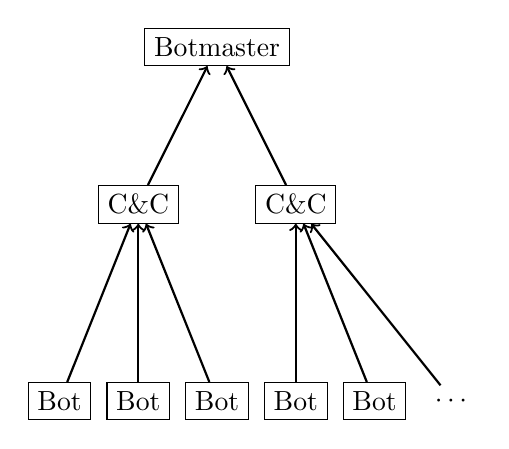
\begin{tikzpicture}
    \node[draw] (m1) {Bot};
    \node[draw] (m2) [right of=m1,node distance=1cm] {Bot};
    \node[draw] (m3) [right of=m2,node distance=1cm] {Bot};
    \node[draw] (m4) [right of=m3,node distance=1cm] {Bot};
    \node[draw] (m5) [right of=m4,node distance=1cm] {Bot};

    \node[draw] (m) [above of=m3,node distance=4.5cm] {Botmaster};
    \node[draw] (cc1) [above of=m2,node distance=2.5cm] {C\&C};
    \node[draw] (cc2) [above of=m4,node distance=2.5cm] {C\&C};

    \draw[->,thick] (m1) -- (cc1);
    \draw[->,thick] (m2) -- (cc1);
    \draw[->,thick] (m3) -- (cc1);
    \draw[->,thick] (m4) -- (cc2);
    \draw[->,thick] (m5) -- (cc2);
    \node (dots) [right of=m5,node distance=1cm] {$\cdots$};
    \draw[->,thick] (dots) -- (cc2);

    \draw[->,thick] (cc1) -- (m);
    \draw[->,thick] (cc2) -- (m);
\end{tikzpicture}
\caption{Botnet C\&C for a centralized botnet with multiple C\&C centers.}
\label{fig:lit-review:botnets:centralized-multiple}
\end{figure}

Although most botnets use IRC or HTTP to communicate directly, the botnet
designed for this paper will communicate over a social network.  This concept
has been discussed in some previous work, for example in \cite{twitter-botnet},
a method of C\&C over Twitter is discussed, however the commands are sent
directly as the content of the tweets instead of by using a covert channel.  A
botnet has been designed to use steganography over a online social network
\cite{stegobot}, but it uses image steganography to embed messages in the images
posted normally by the victim.  It requires that other bots in the botnet be on
computers socially connected to the victim via the online social network.

\section{Methodology}
\label{cha:methodology}

\subsection{Twitter Covert Channel}
\label{sec:methodology:twittercc}

\subsubsection{The Stego System}
\label{subsec:methodology:twittercc:stego}

To perform the botnet command and control communication, a covert channel
(stego system) that communicates using the Twitter social network has been
developed.  This covert channel is similar to Desoky's \cite{nostega} noiseless
steganography and utilizes the cover generation paradigm, however there are some differences.
Even in the noiseless steganography systems, the secret messages are
usually embedded in to the actual data of the cover objects.  For example, in
graph steganography, the plotted data contains the secret message.  In this
system, where the cover objects are tweets, the secret message is not contained
in the data of the tweet (the text), instead it is contained in the
\emph{metadata} of the tweet (the length).  Metadata refers to ``data about
data.''  All data has some metadata associated with it, but this metadata is not
explitictly stored.  It is inferred from the existing data.  The tweet's data is
the text.  The tweet also has metadata such as the time it was posted, the user
account, and the length of the text posted.  Additional metadata could include
the letter frequencies of the posted text or the number of spaces in the text.

Because this system differs from existing steganographic systems, we will
define the parts of this system as follows:

\begin{enumerate}
  \item The set of possible cover messages, $\mathcal{X}^*$, is the set of
  possible tweets, which is the set of messages of up to 140
  UTF-8\footnote{\url{https://dev.twitter.com/docs/counting-characters}}
  characters.
  \item The set of possible secret messages, $\mathcal{M}$, can be defined as
  $\Sigma^*$, where the $\Sigma$ notation is taken from the formal languages
  domain, and refers to an alphabet of symbols, where the symbols can be
  arbitrarily defined.  For example, one implementation may use $\Sigma = \{a,
  b, c, \ldots, z\}$ (the English alphabet).
  \item The set of possible keys, $\mathcal{K}$, is the set of numbers that can
  be valid pseudo-random keys for the implementation.  In our case,
  the implementation uses the Java programming language's
  \ttf{java.util.Random}\footnote{\url{http://docs.oracle.com/javase/8/docs/api/java/util/Random.html}}
  class, which uses 48 bit keys.
  \item The \ttf{Embed} and \ttf{Generate} functions are combined.
  In our implementation we generate reasonable cover messages to have appropriate
  metadata that contains the secret message.
  \item The \ttf{Extract} function will also require a \ttf{Decode} step,
  described below.
  \item For convenience, we will also use the following notation for the set of
  natural numbers up to 140: $\tl = \{1, 2, \ldots, 140\}$.  Similarly, if
  we use $\mathbb{N}_n$, it means the natural numbers from 1 to $n$.  Unless
  otherwise stated, we assume $0 \not\in \mathbb{N}$.
\end{enumerate}

The overall system is shown in figure \ref{fig:twittercc}, where the numbered
components were implemented for the channel.

\begin{figure}
\centering
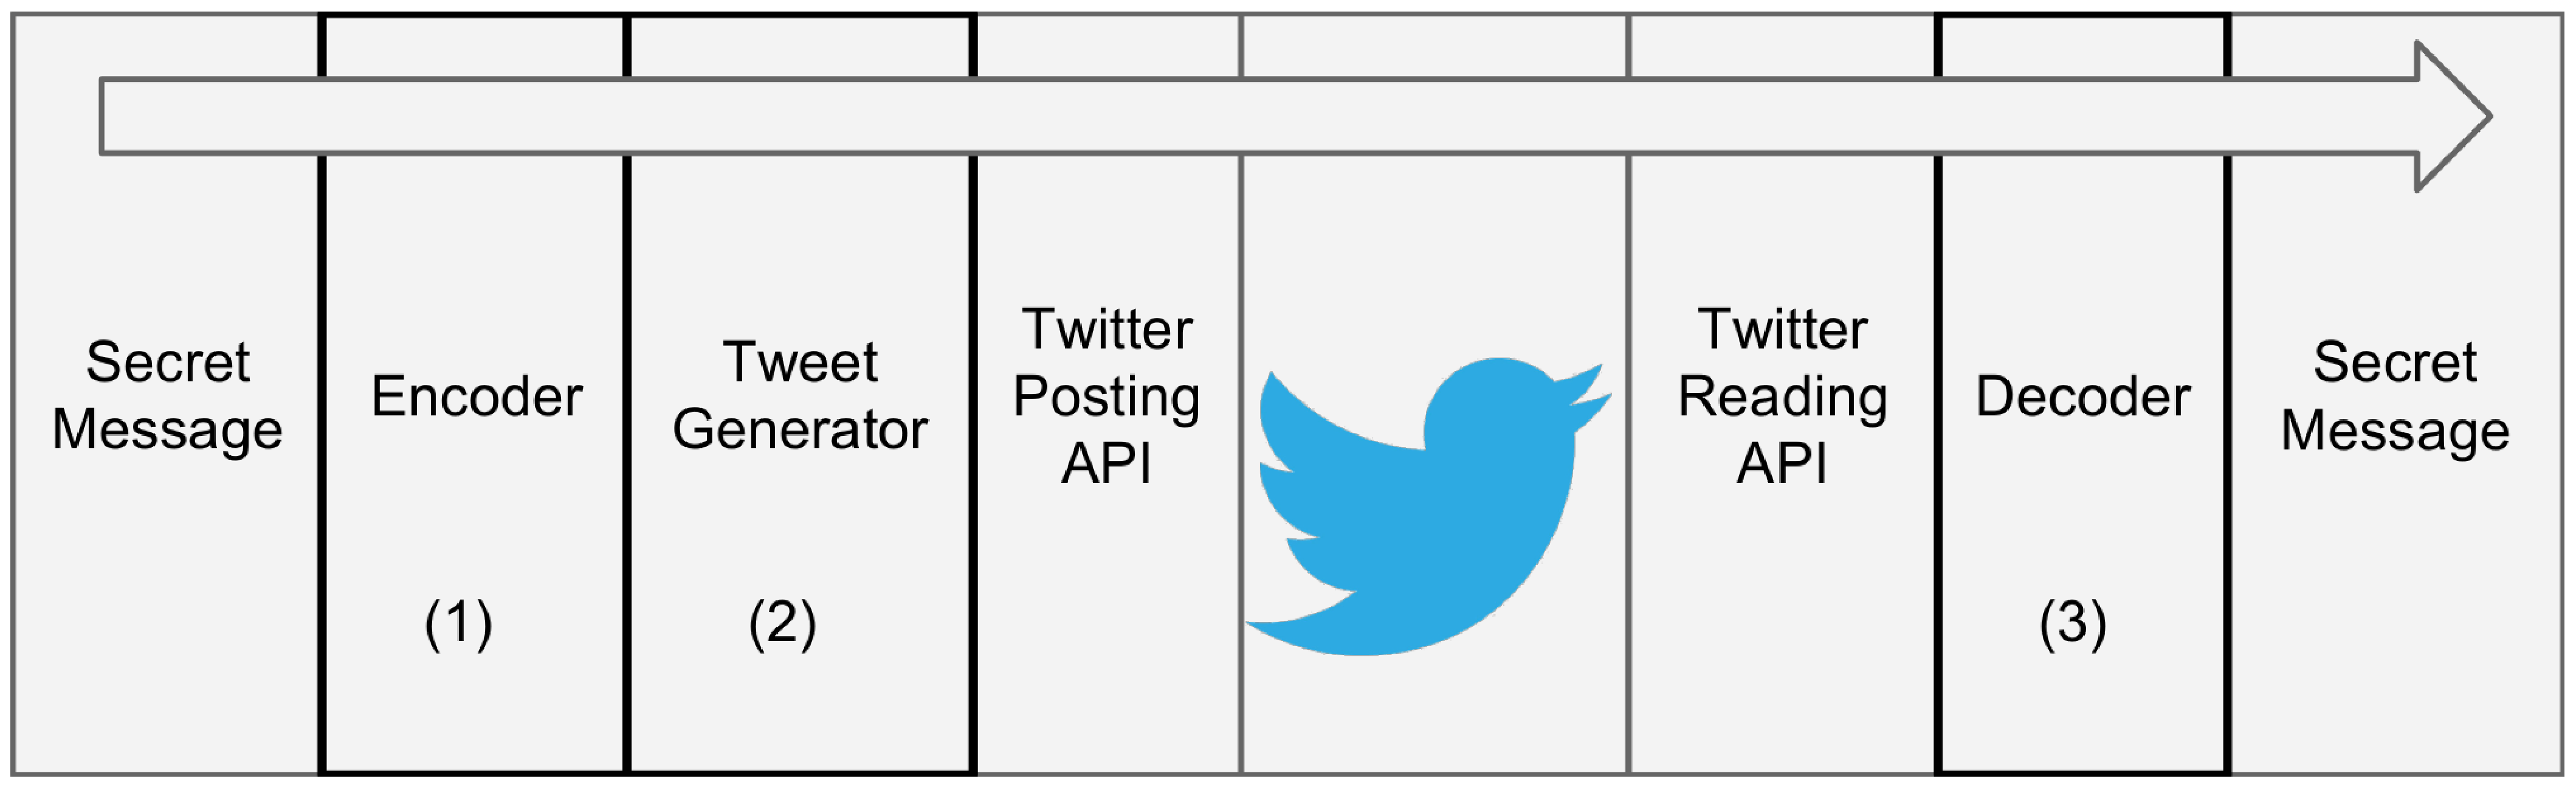
\includegraphics[width=\columnwidth]{twittercc.eps}
\caption{Overview of Twitter covert channel, where the numbered
components were implemented for the channel.}
\label{fig:twittercc}
\end{figure}

The secret message is embedded by utilizing the \emph{length} of the posted
tweets, by character count.  Because a tweet can have a length of up to 140
characters, the length value can store just over 7 bits of information per
tweet.  However, embedding 7 bits of information per tweet is not reasonable in
practice.  Certain length tweets rarely appear on Twitter so seeing, for
example, many tweets of length one or two on a single account would be
suspicious.  To solve these problems, we can use a one-to-many encoding
technique to hide information in the tweet lengths.  We will modify
the normal stego system definition to include the following functions:
\ttf{Encode}: $\mathcal{M} \times \mathcal{K} \rightarrow \tl$ and \ttf{Decode}:
$\tl \times \mathcal{K} \rightarrow \mathcal{M}$.  

\begin{figure}
\centering
\resizebox {\columnwidth} {!} {
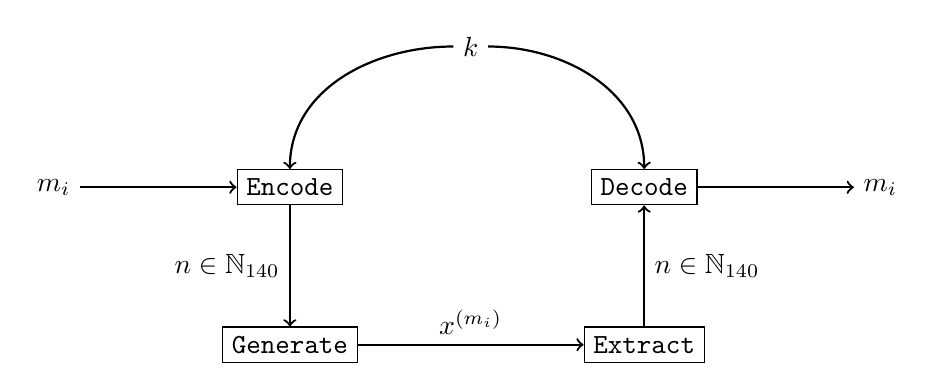
\begin{tikzpicture}
\node (m0) {$m_i$};
\node[draw] (encode) [right of=m0,node distance=3cm] {\ttf{Encode}};
\node[draw] (generate) [below of=encode,node distance=2cm] {\ttf{Generate}};
\node[draw] (extract) [right of=generate,node distance=4.5cm] {\ttf{Extract}};
\node[draw] (decode) [above of=extract,node distance=2cm] {\ttf{Decode}};
\draw[->,thick] (generate) -- (extract) node[pos=.5,above] (xm) {$x^{(m_i)}$};
\draw[->,thick] (encode) -- (generate) node[pos=.5,left] {$n \in \tl$};
\node (k) [above of=xm,node distance=3.5cm] {$k$};
\node (m1) [right of=decode,node distance=3cm] {$m_i$};
\draw[->,thick] (m0) -- (encode);
\draw[->,thick] (extract) -- (decode) node[pos=.5,right] {$n \in \tl$};
\path[->,thick] (k.west) edge [out=180,in=90] (encode.north);
\path[->,thick] (k.east) edge [out=0,in=90] (decode.north);
\draw[->,thick] (decode) -- (m1);
\end{tikzpicture}
}
\caption{Modified stego system diagram for Twitter covert channel.}
\label{fig:stego-twittercc}
\end{figure}

The modified stego system definition is shown in figure
\ref{fig:stego-twittercc}.  A message $m \in \mathcal{M}$ is broken up in to
symbols of $\Sigma$: $m_1m_2\ldots m_a$.  Each symbol $m_i$ is mapped to one of
several possible values using \ttf{Encode} along with the appropriate key $k$ to generate $n
\in \tl$, the appropriate tweet length value to use for this piece of the
message.  This value is passed to \ttf{Generate}, which generates a plausible
cover message $x^{(m_i)} \in \mathcal{X^*}$ to be posted to Twitter.  The
\ttf{Extract} function reads the posted tweets and calculates the length $n$ of
each tweet.  This value is passed to \ttf{Decode} along with the original key
$k$ to reconstruct the original message $m$ piece by piece.  This design assumes
that $\lvert\Sigma\rvert \leq 140$, and in fact, smaller alphabets should
improve the security of the channel.  A smaller alphabet allows mapping each symbol to more
possible length values, so repetitions of each length value are less likely.  We
will now present a simplified example to show the process of the stego
system.

\begin{example}[Encoding Table Generation]
\label{ex:methodology:twittercc:stego:encoding}
In this \\example, we will show the process for generating the encoding table.
Instead of using $\tl$ (all possible length values), we will use a reduced output
alphabet of $\mathbb{N}_{10}$ (1, 2, \ldots, 10) with an equal distribution.
For the input alphabet, we will use $\Sigma = \left\{a, b\right\}$ with an equal
distribution.

\begin{center}
\resizebox {\columnwidth} {!} {
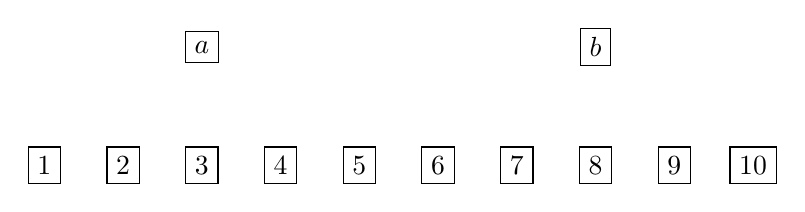
\begin{tikzpicture}
\node[draw] (a) {$a$};
\node[draw] (b) [right of=a,node distance=5cm] {$b$};

\node[draw] (3) [below of=a,node distance=1.5cm] {3};
\node[draw] (4) [right of=3,node distance=1cm] {4};
\node[draw] (5) [right of=4,node distance=1cm] {5};
\node[draw] (6) [right of=5,node distance=1cm] {6};
\node[draw] (7) [right of=6,node distance=1cm] {7};
\node[draw] (8) [right of=7,node distance=1cm] {8};
\node[draw] (9) [right of=8,node distance=1cm] {9};
\node[draw] (10) [right of=9,node distance=1cm] {10};
\node[draw] (2) [left of=3,node distance=1cm] {2};
\node[draw] (1) [left of=2,node distance=1cm] {1};
\end{tikzpicture}
}
\end{center}

First, choose one element of the output alphabet for each element
of $\Sigma$.  This guarantees that at least one output symbol will be mapped to
each input symbol.  Remove the chosen values of the output alphabet as options for
future choices.


\begin{center}
\resizebox {\columnwidth} {!} {
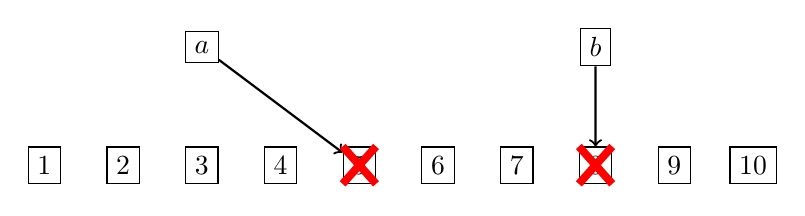
\begin{tikzpicture}
\node[draw] (a) {$a$};
\node[draw] (b) [right of=a,node distance=5cm] {$b$};

\node[draw] (3) [below of=a,node distance=1.5cm] {3};
\node[draw] (4) [right of=3,node distance=1cm] {4};
\node[draw] (5) [right of=4,node distance=1cm] {5};
\node[draw] (6) [right of=5,node distance=1cm] {6};
\node[draw] (7) [right of=6,node distance=1cm] {7};
\node[draw] (8) [right of=7,node distance=1cm] {8};
\node[draw] (9) [right of=8,node distance=1cm] {9};
\node[draw] (10) [right of=9,node distance=1cm] {10};
\node[draw] (2) [left of=3,node distance=1cm] {2};
\node[draw] (1) [left of=2,node distance=1cm] {1};

\draw[->,thick] (a) -- (5);
\draw[->,thick] (b) -- (8);

\draw[red, line width=1mm]
(5.south west) -- (5.north east)
(5.south east) -- (5.north west);

\draw[red, line width=1mm]
(8.south west) -- (8.north east)
(8.south east) -- (8.north west);
\end{tikzpicture}
}
\end{center}

Now, choose one element from both sets probabilistically based on the weights.

\begin{center}
\resizebox {\columnwidth} {!} {
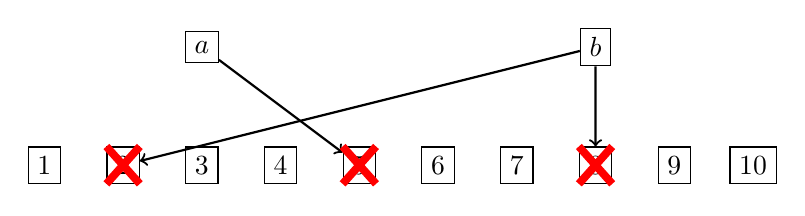
\begin{tikzpicture}
\node[draw] (a) {$a$};
\node[draw] (b) [right of=a,node distance=5cm] {$b$};

\node[draw] (3) [below of=a,node distance=1.5cm] {3};
\node[draw] (4) [right of=3,node distance=1cm] {4};
\node[draw] (5) [right of=4,node distance=1cm] {5};
\node[draw] (6) [right of=5,node distance=1cm] {6};
\node[draw] (7) [right of=6,node distance=1cm] {7};
\node[draw] (8) [right of=7,node distance=1cm] {8};
\node[draw] (9) [right of=8,node distance=1cm] {9};
\node[draw] (10) [right of=9,node distance=1cm] {10};
\node[draw] (2) [left of=3,node distance=1cm] {2};
\node[draw] (1) [left of=2,node distance=1cm] {1};

\draw[->,thick] (a) -- (5);
\draw[->,thick] (b) -- (8);
\draw[->,thick] (b) -- (2);

\draw[red, line width=1mm]
(5.south west) -- (5.north east)
(5.south east) -- (5.north west);

\draw[red, line width=1mm]
(8.south west) -- (8.north east)
(8.south east) -- (8.north west);

\draw[red, line width=1mm]
(2.south west) -- (2.north east)
(2.south east) -- (2.north west);
\end{tikzpicture}
}
\end{center}

Continue this process until all elements of the output alphabet have been
used.

\begin{center}
\resizebox {\columnwidth} {!} {
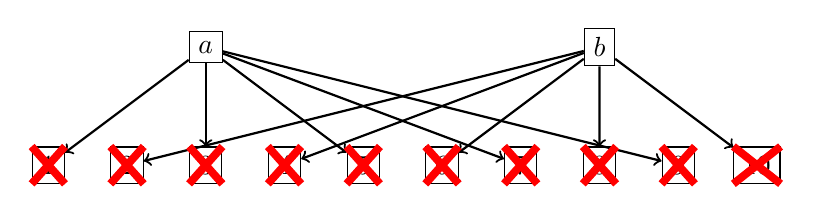
\begin{tikzpicture}
\node[draw] (a) {$a$};
\node[draw] (b) [right of=a,node distance=5cm] {$b$};

\node[draw] (3) [below of=a,node distance=1.5cm] {3};
\node[draw] (4) [right of=3,node distance=1cm] {4};
\node[draw] (5) [right of=4,node distance=1cm] {5};
\node[draw] (6) [right of=5,node distance=1cm] {6};
\node[draw] (7) [right of=6,node distance=1cm] {7};
\node[draw] (8) [right of=7,node distance=1cm] {8};
\node[draw] (9) [right of=8,node distance=1cm] {9};
\node[draw] (10) [right of=9,node distance=1cm] {10};
\node[draw] (2) [left of=3,node distance=1cm] {2};
\node[draw] (1) [left of=2,node distance=1cm] {1};

\draw[->,thick] (a) -- (5);
\draw[->,thick] (b) -- (8);
\draw[->,thick] (b) -- (2);
\draw[->,thick] (a) -- (1);
\draw[->,thick] (a) -- (3);
\draw[->,thick] (a) -- (7);
\draw[->,thick] (a) -- (9);
\draw[->,thick] (b) -- (4);
\draw[->,thick] (b) -- (6);
\draw[->,thick] (b) -- (10);

\draw[red, line width=1mm]
(5.south west) -- (5.north east)
(5.south east) -- (5.north west);

\draw[red, line width=1mm]
(8.south west) -- (8.north east)
(8.south east) -- (8.north west);

\draw[red, line width=1mm]
(2.south west) -- (2.north east)
(2.south east) -- (2.north west);

\draw[red, line width=1mm]
(1.south west) -- (1.north east)
(1.south east) -- (1.north west);

\draw[red, line width=1mm]
(3.south west) -- (3.north east)
(3.south east) -- (3.north west);

\draw[red, line width=1mm]
(4.south west) -- (4.north east)
(4.south east) -- (4.north west);

\draw[red, line width=1mm]
(6.south west) -- (6.north east)
(6.south east) -- (6.north west);

\draw[red, line width=1mm]
(7.south west) -- (7.north east)
(7.south east) -- (7.north west);

\draw[red, line width=1mm]
(9.south west) -- (9.north east)
(9.south east) -- (9.north west);

\draw[red, line width=1mm]
(10.south west) -- (10.north east)
(10.south east) -- (10.north west);
\end{tikzpicture}
}
\end{center}

After all elements from the output alphabet have been used, the encoding table
is composed of all of the choices made:

\begin{center}
\begin{tabular}{|c|c|}
\hline
Symbol & Possible Length Values \\
\hline
$a$ & 1, 3, 5, 7, 9 \\
\hline
$b$ & 2, 4, 6, 8, 10 \\
\hline
\end{tabular}
\end{center}
\end{example}

\begin{example}[Simple Message Encoding Example]
In this example, we will use tweet lengths up to 10, i.e.\ we will use
$\mathbb{N}_{10} = \{1, 2, \ldots, 10\}$ instead of $\tl$.  We will use $\Sigma
= \{a, b\}$ and $\mathcal{X}^* = \{x\}^+$, i.e.\ secret messages will be composed
of combinatiosn of $a$ and $b$ and cover messages will be strings of $x$.

Suppose we want to send the secret message $m = abba$ using the simple
\ttf{Encode} map from example \ref{ex:methodology:twittercc:stego:encoding}.
First, the message
is broken in to the sequence of symbols $a, b, b, a$.  The \ttf{Encode} function
will then map each symbol to a possible length value, e.g.\ 3, 6, 2, 3.  Note
that because each input symbol from $\Sigma$ can map to more than one length
value from $\mathbb{N}_{10}$, the same symbol may or may not be mapped to the
same length value in any given message.  The \ttf{Generate} function will then
create cover messages that match these length values from the set of possible
cover messages $\mathcal{X}^*$: $xxx, xxxxxx, xx, xxx$.  Each cover message
would then be posted to a Twitter account in the order of the original secret
message.  The \ttf{Extract} function on the recipient's side would then take the
tweets in the posted (chronological) order, returning the length values 3, 6, 2,
3.  The \ttf{Decode} function can then apply the same map as the \ttf{Encode}
function and reconstruct the original message $abba$.
\end{example}

This system is generic in that it can be used with many possible input
alphabets, e.g.\ the  English alphabet or
arbitrary half-byte values (0x0, 0x1, \ldots, 0xF).  The English alphabet
allows sending simple messages.  The half-byte alphabet allows sending arbitrary
binary data by splitting each byte of the input data in half and sending each
half as one symbol of the message.  It is impossible to send an entire byte in
one message using this system because the maximum tweet length is only 140
characters.  We chose half-bytes because it is easy to deconstruct and
reconstruct the original bytes and because it is a relatively small alphabet
with only 16 symbols, so it is possible to map each input symbol to almost 10
different tweet length values.  To obtain symbol frequencies for the half-byte
values, it would be best to empirically sample the types of data being sent
across the channel because, in general, each value would likely have an equal
weight.  If the specific type of data being sent is biased toward certain byte
values, that should be considered when weighting the alphabet.

The botnet command and control diagram for this system resembles the diagram
for a centralized botnet, as shown in figure \ref{fig:methodology:twittercc:botnet-diagram}.
A botmaster controls one or more Twitter accounts that have tweets containing
the commands and the bots read from these accounts.

\begin{figure}
\centering
\resizebox {\columnwidth} {!} {
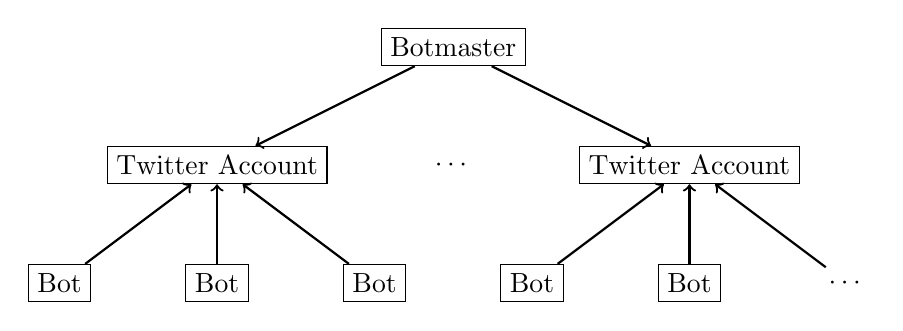
\begin{tikzpicture}
    \node[draw] (m1) {Bot};
    \node[draw] (m2) [right of=m1,node distance=2cm] {Bot};
    \node[draw] (m3) [right of=m2,node distance=2cm] {Bot};
    \node[draw] (m4) [right of=m3,node distance=2cm] {Bot};
    \node[draw] (m5) [right of=m4,node distance=2cm] {Bot};

    \node[draw] (cc1) [above of=m2,node distance=1.5cm] {Twitter Account};
    \node (ccdots) [right of=cc1,node distance=3cm] {$\cdots$};
    \node[draw] (cc2) [above of=m5,node distance=1.5cm] {Twitter Account};
    \node[draw] (m) [above of=ccdots,node distance=1.5cm] {Botmaster};

    \draw[->,thick] (m1) -- (cc1);
    \draw[->,thick] (m2) -- (cc1);
    \draw[->,thick] (m3) -- (cc1);
    \draw[->,thick] (m4) -- (cc2);
    \draw[->,thick] (m5) -- (cc2);
    \node (dots) [right of=m5,node distance=2cm] {$\cdots$};
    \draw[->,thick] (dots) -- (cc2);

    \draw[->,thick] (m) -- (cc1);
    \draw[->,thick] (m) -- (cc2);
\end{tikzpicture}
}
\caption{The botnet C\&C diagram for the system.}
\label{fig:methodology:twittercc:botnet-diagram}
\end{figure}

\subsubsection{The Tweet Generator}
\label{subsec:methodology:twittercc:tweet-gen}

The \ttf{Generate} function is one of the most challenging aspects of this type
of stego system.  As discussed in \cite{steganalysis}, generating appropriate
and plausible cover messages for a stego system is a non-trivial problem.  In this
system, the generator must be capable of generating messages that can convince a
reader of the Twitter account page that they are viewing regular tweets.  This
component has the largest impact on the detectability of the channel.  In
essence, the generator must pass a simplified Turing test.  Twitter bots are not
a new phenomenon, and in fact several bots were created that successfully
convinced other users that they were real people \cite{realboy}.  Additionally,
chat bots exist, such as Cleverbot\footnote{\url{http://www.cleverbot.com/}}
which are reasonably successful \cite{dialogue-system}.  However, aside from
competent English skills, the generator must utilize the ``language of Twitter''
that consists of many
retweets\footnote{\url{https://support.twitter.com/articles/77606-faqs-about-retweets-rt}}
and
hashtags\footnote{\url{https://support.twitter.com/articles/49309-using-hashtags-on-twitter}}.
We consider a strong generator out of the scope of this work, but we leverage the collected Twitter data to create a Twitter language model
based on tweet contents that can be used to generate new tweets.

\subsubsection{Posting to Twitter}
\label{subsec:methodology:twittercc:posting}

Along with the \ttf{Encode}, \ttf{Generate}, \ttf{Extract}, and \ttf{Decode}
functions, we need a system that can post to Twitter.
This is easy to do for testing purposes thanks to Twitter's official
API\footnote{\url{https://dev.twitter.com/docs/api}} and a third party Java
library, Twitter4J\footnote{\url{http://twitter4j.org}}.
For a real botnet scenario, the implementer would likely write their own system
that uses raw HTTP requests because the Twitter API requires authentication of
every call, detects the posting method, and limits the number of posts allowed
for each account.  However, because this would violate Twitter's terms of use, we
will only post tweets using the official API and abide by all limitations
for testing.  Now that the rest of the components have been explained, a more
complete example will be presented.

\begin{example}[Complete Example]
In this example, we will use the full range of tweet lengths $\tl$.  We will use
$\Sigma = \{A, B, \ldots, Z\}$ (the English alphabet), and $\mathcal{X}^*$ as a
pre-constructed list of various proverbs and phrases of lengths ranging from one
to 140.  The \ttf{Generate} function will lookup an appropriate phrase for each
length message provided by the \ttf{Encode} function.  Table
\ref{tab:real-encode} shows a portion of a generated encoding map from English letters to
tweet lengths.  The weights shown in the second column are taken as letter
frequencies\footnote{\url{http://www.math.cornell.edu/~mec/2003-2004/cryptography/subs/frequencies.html}}.
Those weights were used to decide the number of entries for each letter in the
third column.  

Suppose we want to send the message $FOO$.  First, the message is separated in
to the sequence of symbols $F, O, O$.  Each is passed to the \ttf{Encode}
function, which chooses appropriate lengths, e.g.\ 61, 35, 121.  The
\ttf{Generate} function then generates tweets and they are posted to Twitter, as
shown in figure \ref{fig:twitter-posts-foo}.  The figure should be read from
bottom up, because the newer messages are posted on top of the older messages.
The account shown is a test account created for this work.  The recipient then
reads these tweets, obtains the lengths, then uses \ttf{Decode} with the same
table as was used for the \ttf{Encode} process to get the original message.
\end{example}

\begin{table}
\centering
\begin{tabular}{|c|c|p{5.2cm}|}
\hline
Symbol & Weight & Encoding \\
\hline
A & 14810 & 32, 16, 19, 131, 84, 37, 106, 140, 76, 111\\
\hline
B & 2715 & 105, 138, 67 \\
\hline
C & 4943 & 75, 36, 125, 46, 62\\
\hline
F & 4200 & 17, 122, 61, 87\\
\hline
 \ldots & \ldots & \ldots \\
\hline
O & 14003 & 35, 121, 43, 107, 92, 12\\
\hline
 \ldots & \ldots & \ldots \\
\hline
\end{tabular}
\caption{Sample encoding map example for a few English alphabets.}
\label{tab:real-encode}
\end{table}

\begin{figure}
\centering
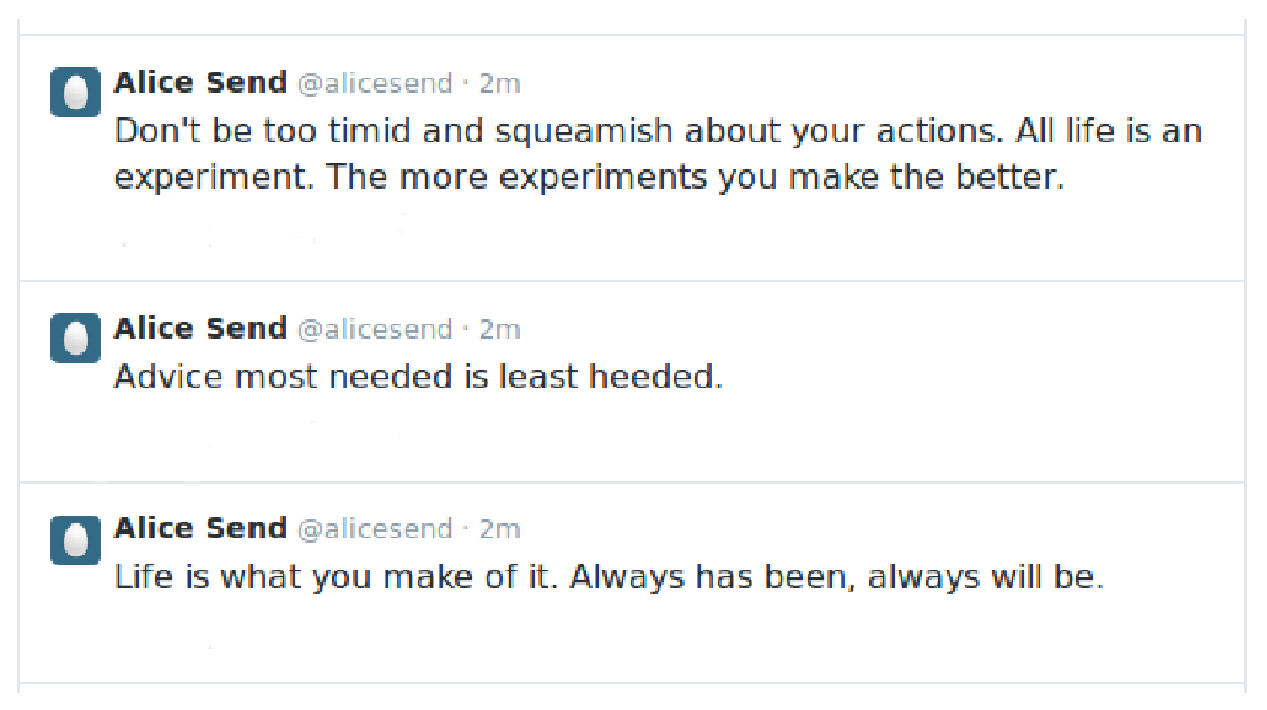
\includegraphics[width=\columnwidth]{foo_test.eps}
\caption{Example showing posted tweets for secret message $FOO$.}
\label{fig:twitter-posts-foo}
\end{figure}

\subsubsection{The Botnet Command and Control Language}
\label{sec:methodology:botnet-cc-lang}

The stego system described in section \ref{subsec:methodology:twittercc:stego} can be
used with an arbitrary input alphabet as long as its size is not larger than the
tweet length range (up to 140 characters), so for botnet command and control we
have developed a language that can be mapped to tweet lengths and interpreted to
execute botnet commands.  We have included some common botnet commands as described
in \cite{twitter-botnet}.  The weights were decided somewhat arbitrarily, because
in a real scenario the botmaster would tailor the weights based on which
commands they believe that they are likely to send most often.  In this case,
We are assuming the byte values (indices 0 to 15) are more likely, because for
some commands arguments must be sent using these.  We don't assume any single
command is more likely than another.

\begin{table}[h]
\centering
\begin{tabular}{|l|l|p{5cm}|}
\hline
Index & Weight & Description \\
\hline
0 & 25 & Literal hex value 0 \\
\hline
1 & 25 & Literal hex value 1 \\
\hline
2 & 25 & Literal hex value 2 \\
\hline
\ldots & \ldots &\ldots \\
\hline
16 & 5 & Take screenshot \\
\hline
17 & 5 & Shutdown computer \\
\hline
18 & 5 & Reboot computer \\
\hline
19 & 5 & Perform DoS attack to IPv4 address in next 4 bytes sent \\
\hline
20 & 5 & Stop DoS attack \\
\hline
21 & 5 & Download and execute file from address in next $k$ bytes (until delimiter) \\
\hline
22 & 1 & Message delimiter \\
\hline
\end{tabular}
\caption{Botnet command and control language for use with the stego system.}
\label{tab:botnet-cc-lang}
\end{table}

\subsubsection{Username Generation using \\Markov Chains}
\label{sec:methodology:usernames}

It is necessary to have a system for generating user names from an initial
seed so that if the original botmaster account is blocked, they can start
a new account and the bots can also generate the new account name and begin
reading from it.  To do this, we employ Markov chains \cite{Markov-chains}.
The Markov chain being used can generate strings of letters, numbers, and
underscores and is trained using an existing corpus of such text (in our case,
a collection of verified Twitter usernames). 

To use this Markov chain for generating a sequence of usernames, both the
bot and botmaster must have the same initial seed.  Using this seed and the
same type of pseudorandom number generator, the
Markov chains will generate the same sequences as long as both bot and
botmaster follow the same procedure.  First, they need to use the random
number generator to choose a user name length.  Second, they use the Markov
chain with this seed to choose
a starting character.  Finally, they generate enough symbols to fit the
length chosen.  If one performs an action out of order, it will affect
the sequences generated after that action.  For example, if the botmaster
chooses the length first while the bot chooses the starting character first,
the sequence generated from the random number generator will cause each to
generate a potentially different length and starting character.


\section{Evaluation of Results}
\label{cha:evaluation}
\subsection{Tweet Collection}
\label{sec:methodology:data-collection}

Several portions of this paper required collecting data from Twitter.  To
determine the posting rate of tweets of each length, it was necessary to collect
tweets from real accounts.  Therefore, data from
verified\footnote{\url{https://support.twitter.com/articles/119135-faqs-about-verified}
\url{-accounts}}
Twitter accounts was collected.  A verified account is an account that Twitter
has manually verified to be a specific person or brand.  By using verified accounts, this
prevents obtaining data from other bots or fake accounts.  However, it has been
noted that verified accounts may not be a perfect representation of the average
Twitter user, who is not generally a brand or celebrity.  User information stored
includes the username and user ID, a unique integer that Twitter stores for
each user.  A total of 54,114 users were collected.  Additionally, for
creating the Markov chain, tweet content was parsed using a regular expression
from the collected tweets to find username references in the tweets.  In a
tweet, usernames are preceded by an @ symbol.

From the collected user IDs, tweet content, length, unique identifier, and
posting time were collected.  Because of the number of collected users and
the number of tweets posted by each user, during the data collection we only
obtained tweets from 3,709 users.  However, this totaled 7,345,681 tweets.
This data collection was done automatically from a list of verified users that
was obtained from Twitter.  Twitter has a special account with username
\emph{verified} that will follow all verified accounts.  Therefore, we were
able to search for all accounts followed by that special account using the
Twitter API and then begin obtaining tweets posted by each of those accounts.
Not all accounts post in English, some collected data is in other languages
including Portuguese, Spanish, Japanse, and Arabic among others.  In order
to remove these languages, we used the third-party Java library
NGramJ\footnote{\url{http://ngramj.sourceforge.net/index.html}}, which performs
language recognition using n-grams.  An n-gram is a sequence of symbols of length
$n$.  For example, in English a common bigram (2-gram) is \emph{th}.  This library
ranked each tweet according to which language it most resenbled.  We kept only the
tweets where the highest ranking language is English.  This left us with 5,461,009
tweets out of the original 7,345,681.  However, this method is not perfect.
Tweets contain some non-typical English characters in hashtags, names,
misspellings, URLs, etc.  Because of this, the n-gram analysis likely had some
false positives and false negatives.  For example, one tweet had the text
``Vancouver, 9/25'', but the n-gram model marked it as French.  After this
n-gram analysis, tweets were further restricted by checking the character
values in each tweet.  If a tweet contains too many non-ASCII characters,
then it is not likely to be English.  In this case, we removed all tweets that
were 10\% or more non-ASCII characters.  This allows up to approximately 14
non-ASCII characters in a full length tweet.  The final tweet count is 5,011,973.

\subsection{Stego System Evaluation}
\label{sec:evaluation:twittercc}

\subsubsection{Emulab Performance and Reliability Experiment}
\label{subsec:evaluation:twittercc:emulab}

Emulab \cite{emulab-rigorous} is a network testbed and software system designed for testing networked
systems.  It allows experimenters to request a set of physical machines,
or nodes, that
are configured in a specific network configuration as defined by a script
file supplied to the Emulab website.  

The experiment for this paper was performed by generating symbols from a test
alphabet (the English alphabet) and posting
generated tweets using a random text generator and a constructed encoding map.
The input symbols were chosen probabilistically with the weight associated with
their letter frequencies.
The ``botmaster'' acted from a desktop computer outside of the Emulab environment
posting the tweets while the ``bots'' acted from inside an Emulab experimental
setup.  There were five bots in the experiment running Emulab's
\ttf{UBUNTU12-64-STD} operating system image.  The botmaster generated a new
symbol and posted the corresponding tweet every 30 seconds while the bots
performed an HTTP request to the correct Twitter account every 10 seconds
checking for new tweets.  Each time the botmaster posted, it is recorded
to a log file.  Each time the bots read a tweet, they also recorded to a log
file.  Afterwards, the logs were collected to compare the post time with
the retrieval time and also to match each original input symbol with the
decoded symbols from the bots.  Due to a time zone difference between the
botmaster machine and the bots in the Emulab setup, the original time stamps
from the bots appeared one hour later, so one hour was subtracted from their
times when comparing the difference in posting and reading time between the
botmaster and bots.  Figure \ref{fig:evaluation:twittercc:emulab:emulab}
shows the network configuration for the experiment. 

\begin{figure}
\centering
\resizebox {\columnwidth} {!} {
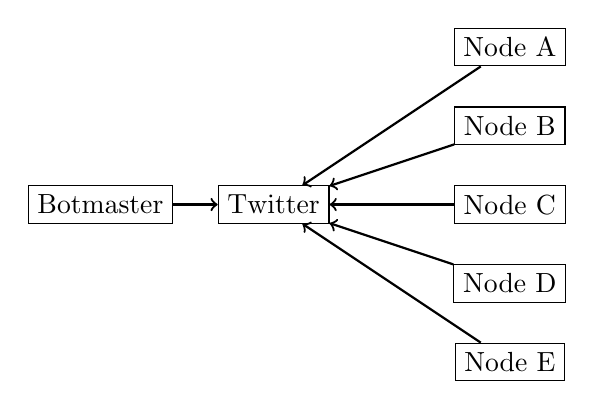
\begin{tikzpicture}
    \node[draw] (botmaster) {Botmaster};
    \node[draw] (twitter) [right of=botmaster,node distance=2.2cm] {Twitter};

    \node[draw] (nodec) [right of=twitter,node distance=3cm] {Node C};
    \node[draw] (nodeb) [above of=nodec,node distance=1cm] {Node B};
    \node[draw] (nodea) [above of=nodeb,node distance=1cm] {Node A};
    \node[draw] (noded) [below of=nodec,node distance=1cm] {Node D};
    \node[draw] (nodee) [below of=noded,node distance=1cm] {Node E};

    \draw[->,thick] (botmaster) -- (twitter);
    \draw[->,thick] (nodea) -- (twitter);
    \draw[->,thick] (nodeb) -- (twitter);
    \draw[->,thick] (nodec) -- (twitter);
    \draw[->,thick] (noded) -- (twitter);
    \draw[->,thick] (nodee) -- (twitter);
\end{tikzpicture}
}
\caption{Diagram for the Emulab experiment network layout.}
\label{fig:evaluation:twittercc:emulab:emulab}
\end{figure}

In the experiment, 100\% of input symbols were correctly decoded by the bots
except for a small set that were off by one.  After examining the data it was
determined that in these cases, the tweets being posted were generated with
a trailing space that was then trimmed by Twitter while posting.  If the tweets
had been generated without spaces, this would not have occurred and so these
cases were dropped from the results.  The average read time in seconds for
each node are shown in table \ref{tab:evaluation:twittercc:emulab:average-read}.
Each node averaged just over five seconds from the botmaster's post to the
bot's read.  This is likely due to the synchronization issues of the botmaster's
posting and the bot's sleep time between reads.  A total of 305 tweets were posted
for this test and 10 of them were dropped for having trailing whitespace.  With
an average transmission time of less than six seconds, the overall transmission
rate is up to 10,800 bytes per day.

\begin{table}
\centering
\begin{tabular}{|c|c|c|c|c|}
    \hline
    Node A & Node B & Node C & Node D & Node E \\
    \hline
    5.725  & 5.644  & 5.600  & 5.912  & 5.888 \\
    \hline
\end{tabular}
\caption{Average read time in seconds for each node.}
\label{tab:evaluation:twittercc:emulab:average-read}
\end{table}

\subsubsection{Capacity}
\label{subsec:evaluation:twittercc:capacity}

There are three major criteria
for stego system evaluation: capacity, steganographic security, and
robustness \cite{steganalysis}.

At the most basic level, the devised stego system can be used to transmit
at most seven bits of information per tweet because a tweet can have a length of
at most 140.  If eight bits were to be transmitted, there would be 256 different
values.  With seven bits, there are 128 different values, so each value can be
sent with a different length tweet.  Therefore, we can state the maximum capacity
as seven bits per tweet.  Tweets are posted to Twitter using UTF-8, which is
a variable length character encoding scheme that is a superset of the ASCII
characters.  UTF-8 characters range from one to four bytes \cite{rfc3629}.
Therefore, the embedding rate will vary depending not only on the length
of the tweet in characters, but also on how many characters per byte are being
used.  The total number of bytes in a tweet is 560, so the total number of
bits is then 4480.  The possible embedding rates are shown in figure
\ref{fig:evaluation:twittercc:capacity:emebedding-rate}.

\begin{figure}
    \centering
    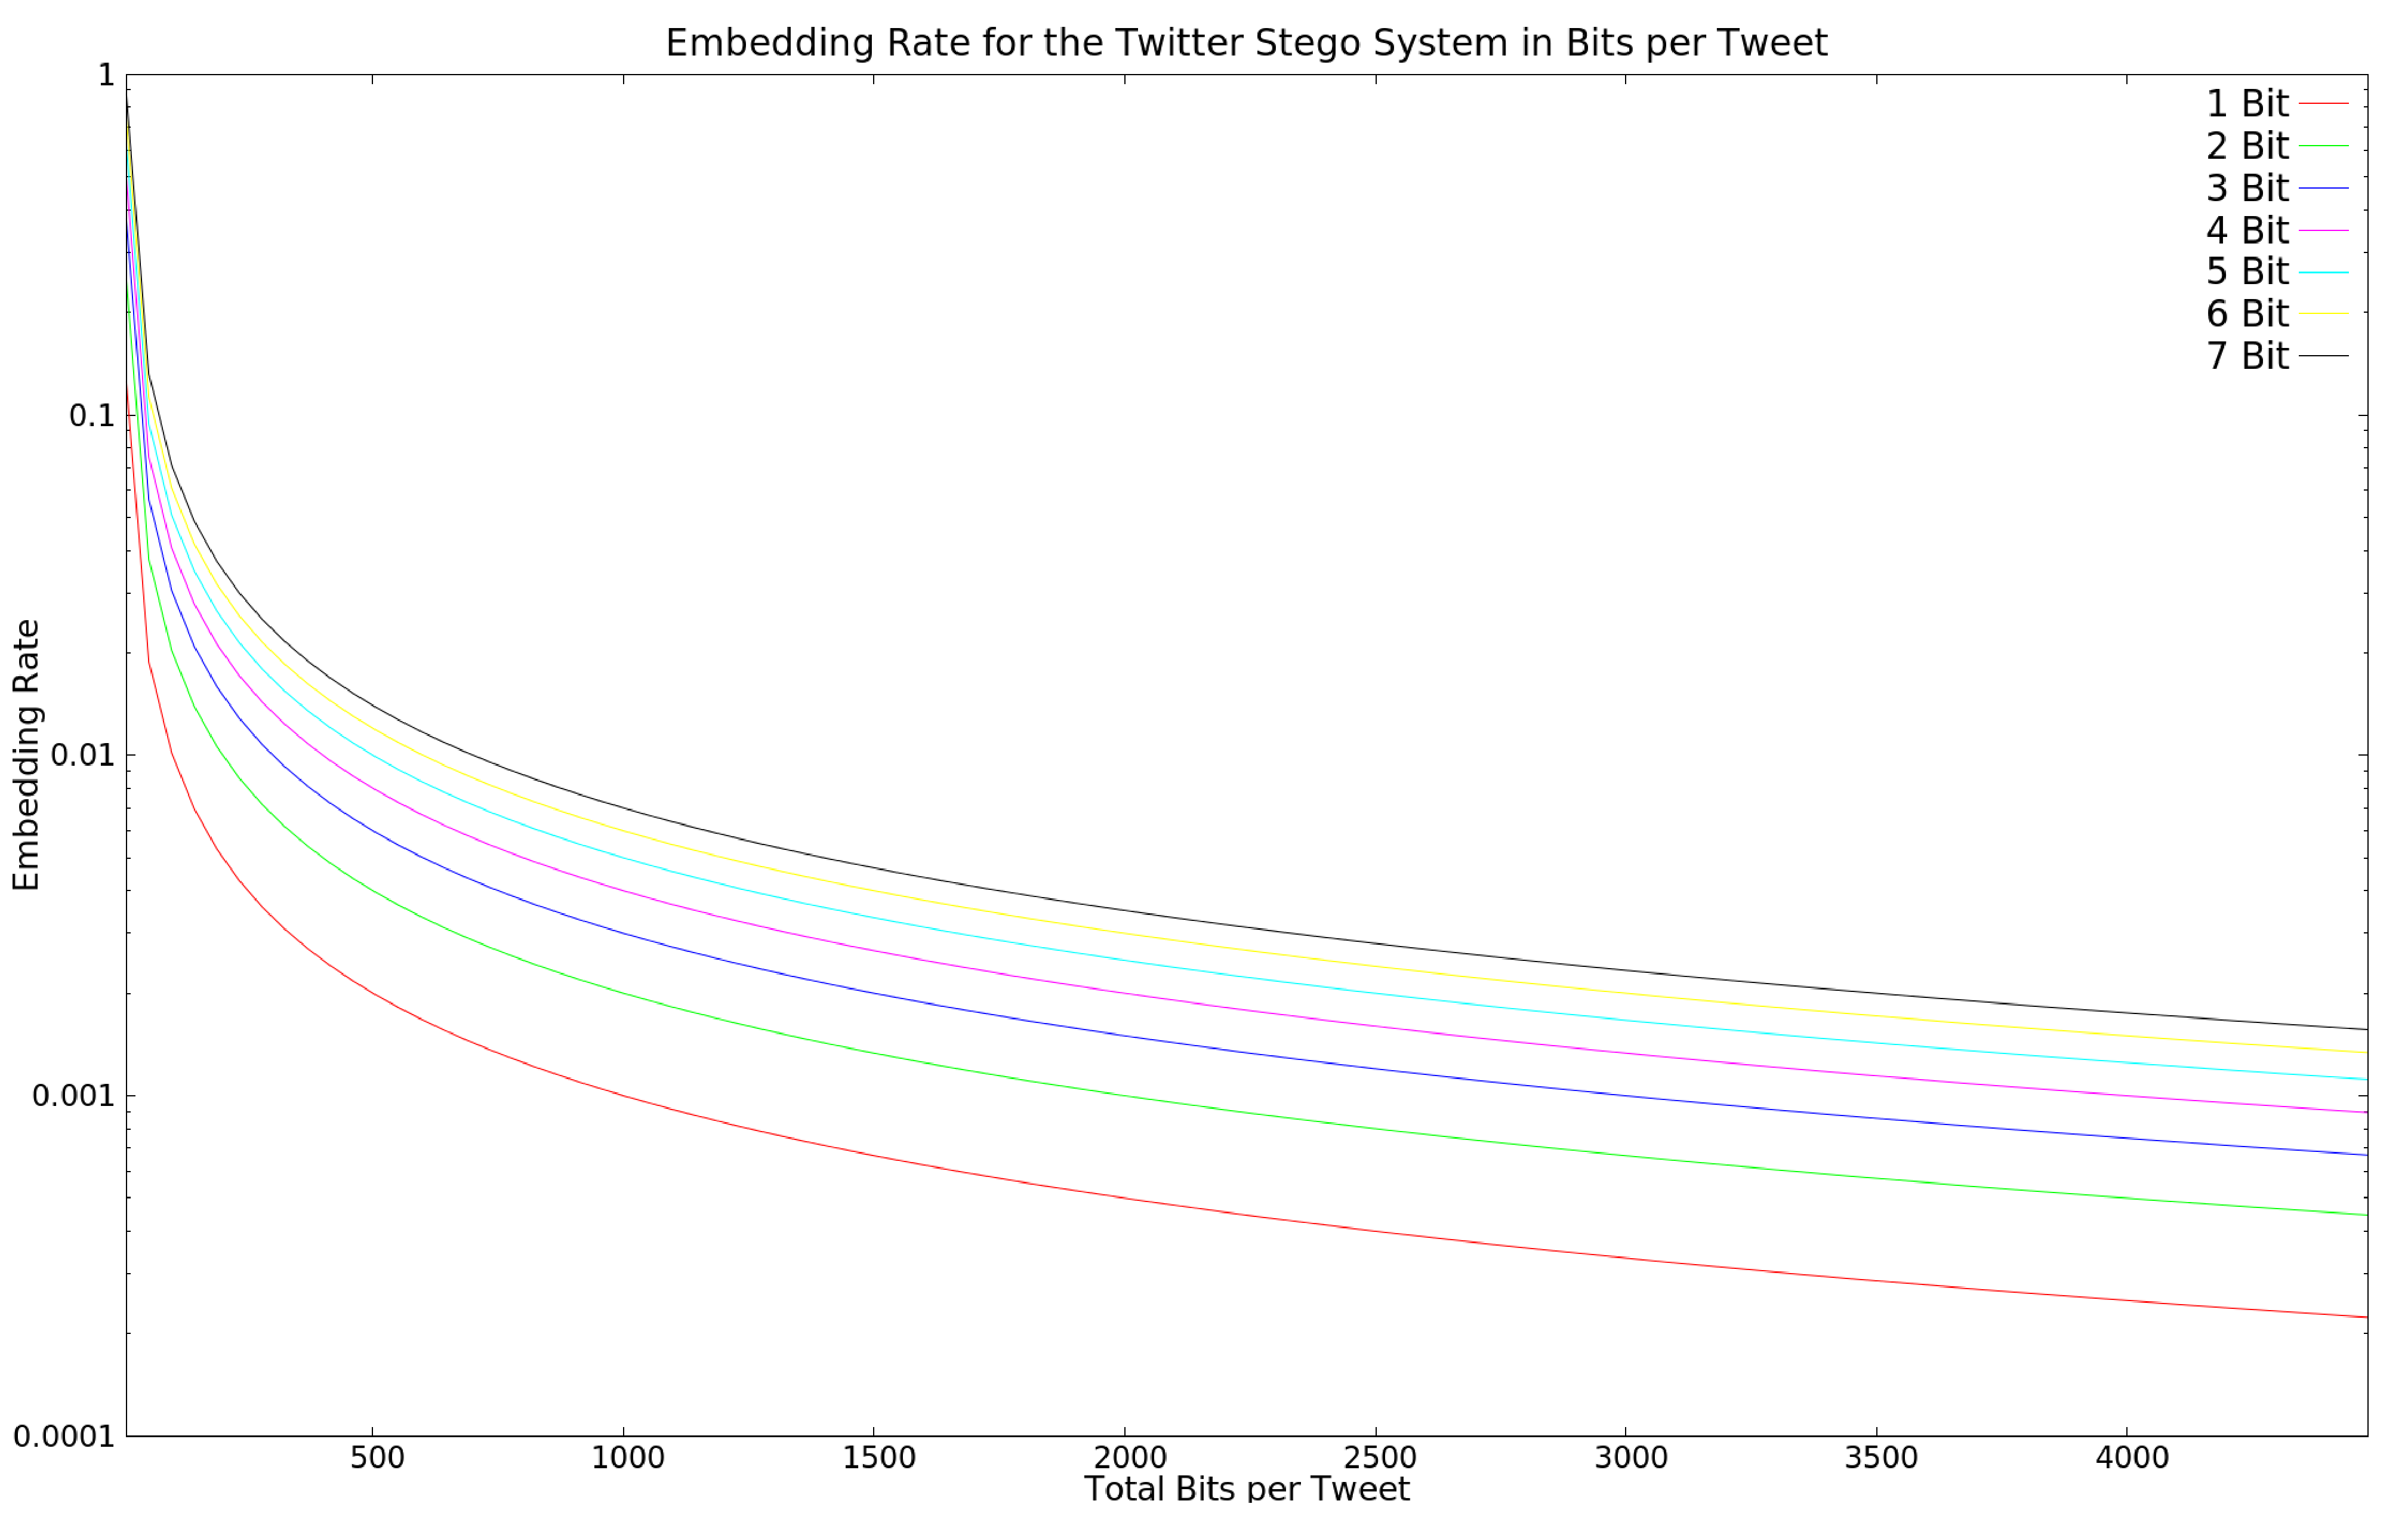
\includegraphics[width=\columnwidth]{embedding-rate.eps}
    \caption{Possible embedding rates for the stego system in bits on a logarithmic scale.}
    \label{fig:evaluation:twittercc:capacity:emebedding-rate}
\end{figure}

Additionally, we must consider how frequently tweets can be posted.  From the
collected Twitter data (see section \ref{sec:methodology:data-collection}),
the time stamp of the tweets was also collected.  For each unique user, the
average number of posts per day was then calculated from this data.  This
data is shown in figure \ref{fig:evaluation:twittercc:capacity:posting-rate}.  In
total, the averege daily posting rate is 8.621 tweets per day.  Therefore, if the
user of the stego system is trying to match real Twitter user posting rates, they
cannot send more than approximately 60 bits of data per day.  If using the system
for botnet command and control, this will allow the botmaster to post a small number
of commands per day.  The botmaster does also have the choice to exceed this
value, but then risks a higher detection rate.  Because the data shows the
average number of tweets posted per day \emph{per account}, that means there
are many accounts that do post more tweets per day.  In this data, there are
several accounts that post on average more than one hundred tweets per day.

\begin{figure}
    \centering
    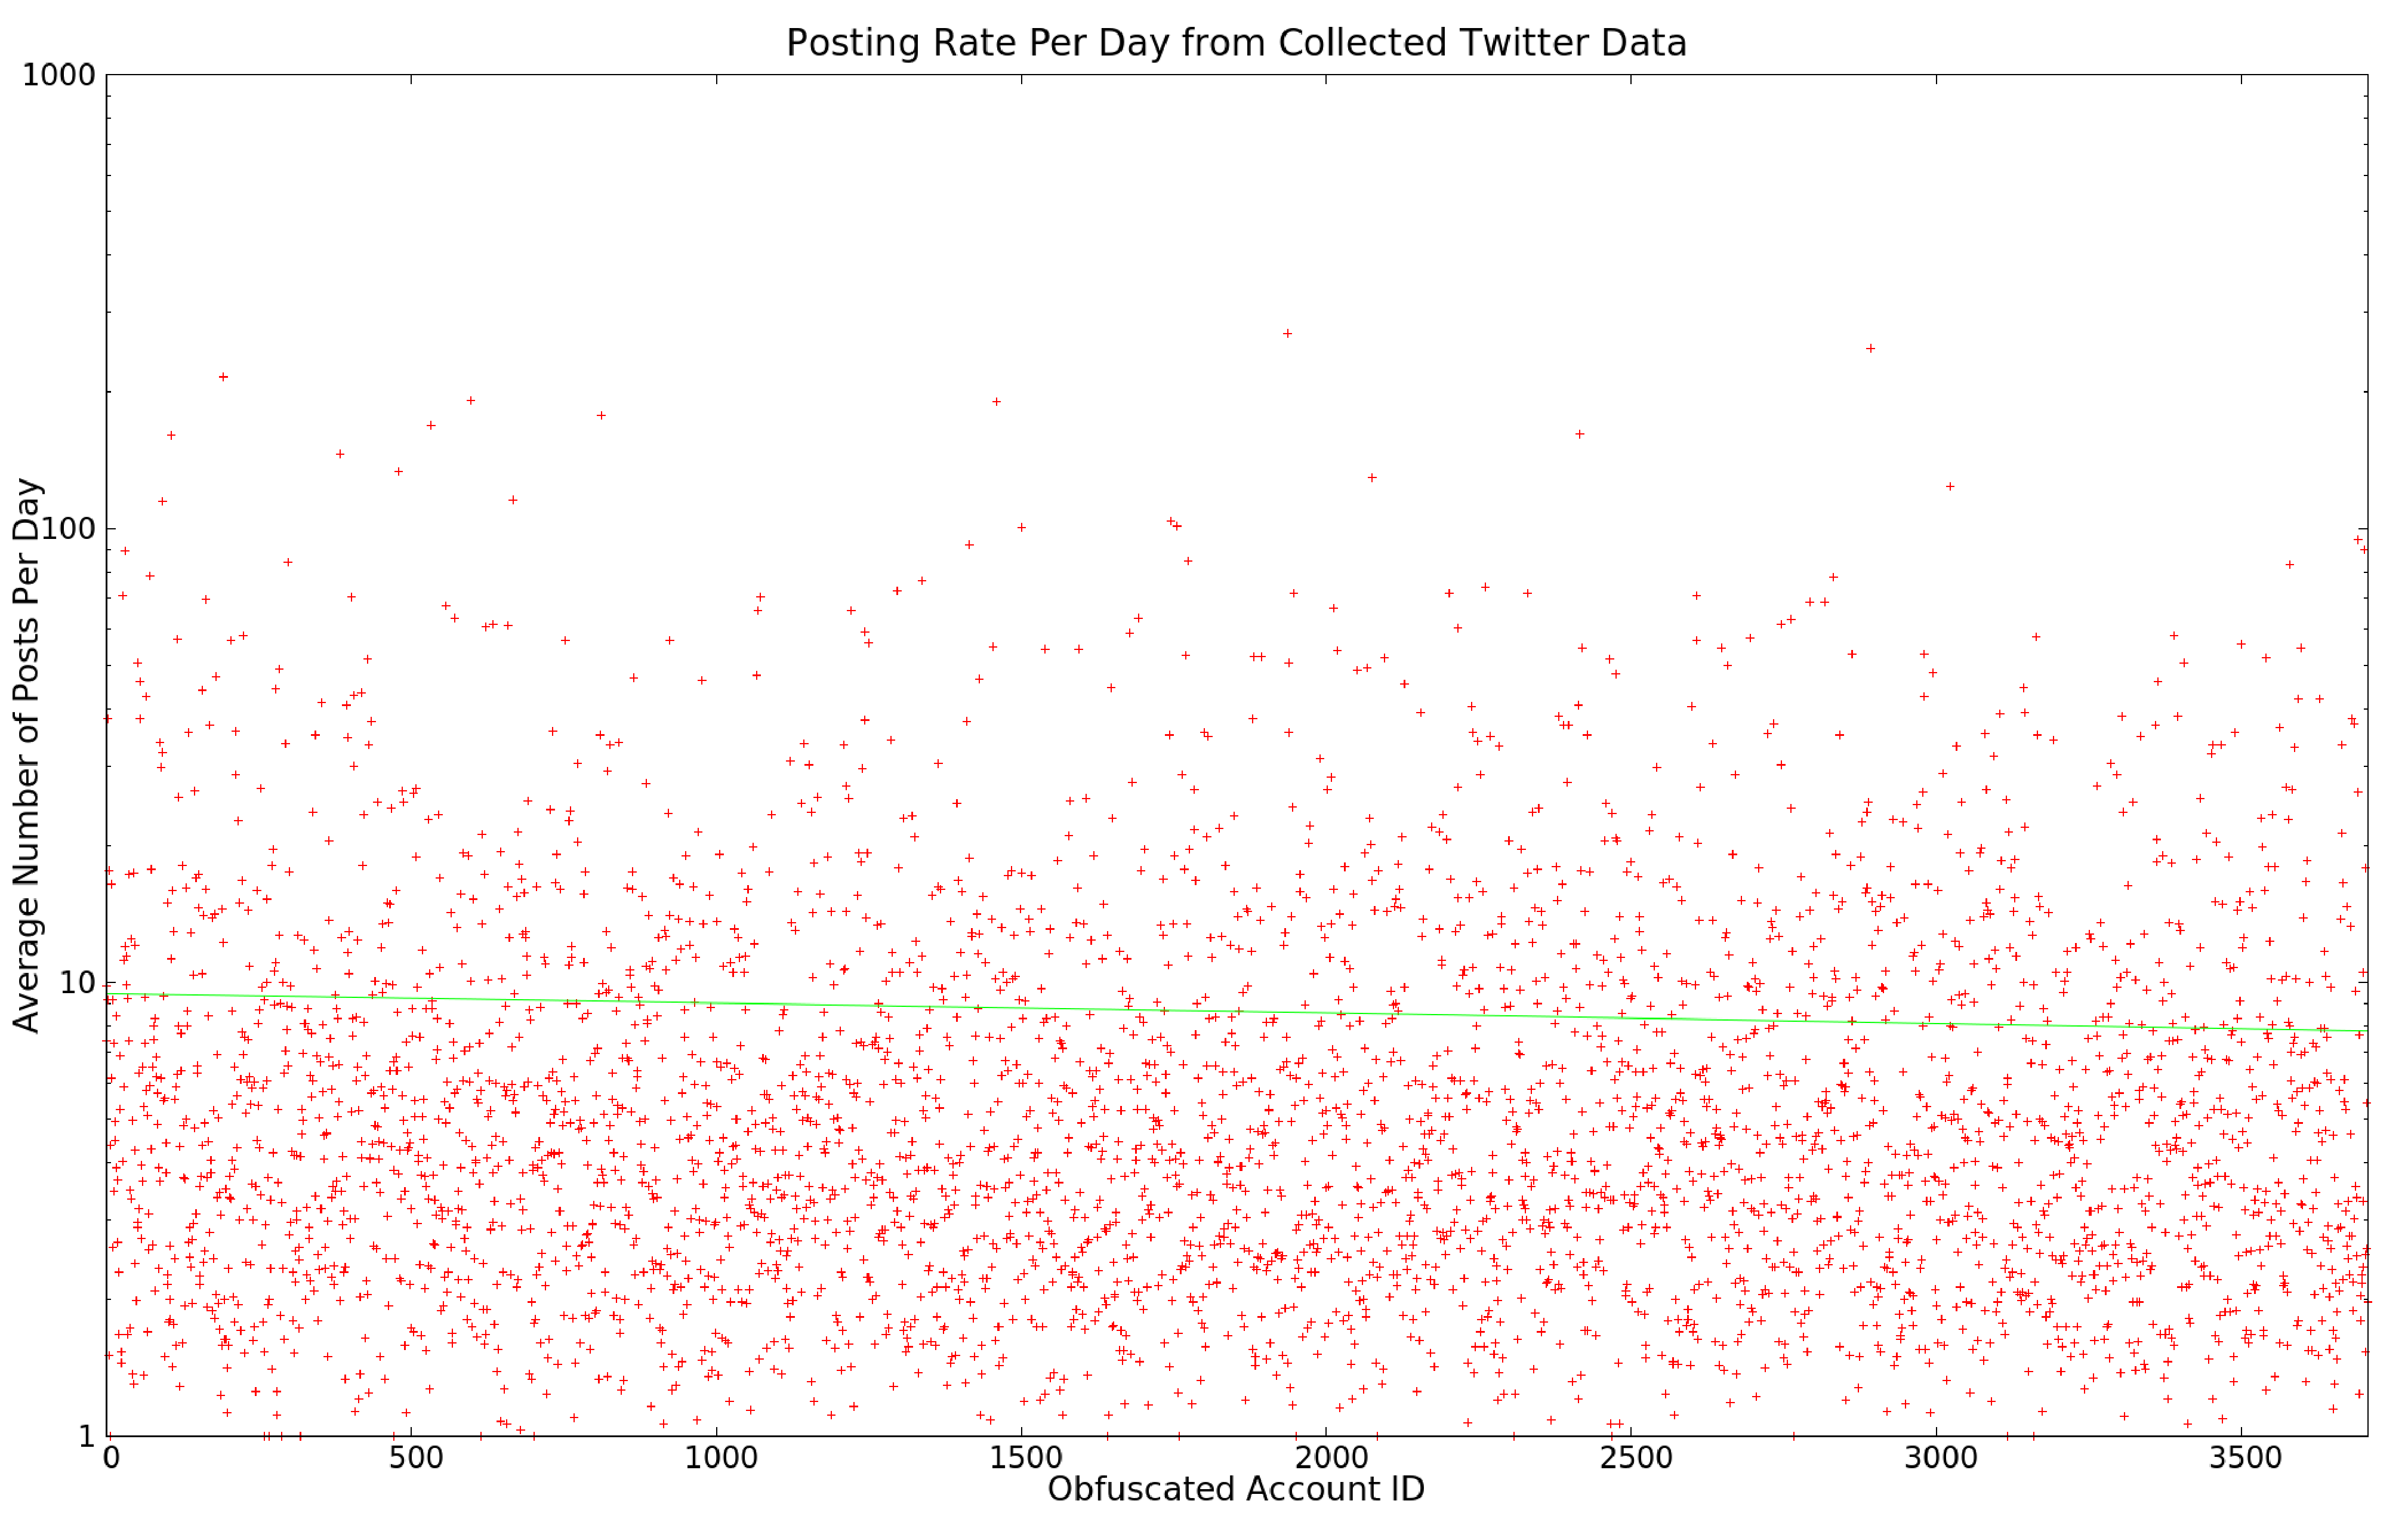
\includegraphics[width=\columnwidth]{posting-rate.eps}
    \caption{Average posting rate in tweets per day on a logarithmic scale.  The green line indicates the mean.}
    \label{fig:evaluation:twittercc:capacity:posting-rate}
\end{figure}

\subsubsection{Steganographic Security}
\label{subsec:evaluation:twittercc:security}

In this stego system we are assuming a \emph{passive warden} model.  In a passive
warden model, an adversary can view each message but cannot modify them.  
The warden must solve the decision problem:
\emph{does this tweet contain a secret message?}  Because our implementation does
not embed any data in to the tweets, most techniques that would be used on a
normal stego system are not sufficient.  The posted tweets appear identical to
any other tweet from a textual perspective.  However, the tweet generation method
is a large determiner of detectability.  It is possible to create the tweets
manually, but if the user wants to send many messages using the stego system
this will be cumbersome.

In order to automate the process, a Twitter bot
program can be used to create the tweets.  An ideal generator would be a
sophisticated Twitter bot that can convince other users that it is human.  This
is similar to passing a Turing test with the Twitter bot.  If an account is
suspected of being a Twitter bot, it does not mean that the communication
has been detected, however it will cause suspicion.  The adversary would have
to recognize that the account is being used to pass secret messages and that
the secret messages are done using the lengths of the tweets.  The adversary
would likely assume that the text somehow contains the secret messages.
If we follow Kerckhoffs' principle \cite{kerckhoffs}, then we must assume the
adversary knows that that the stego system passes messages by tweet lengths.
The two factors that must then be determined are then (i) the account being used for transmission, and (ii) which tweets being posted contain the secret message.


If the adversary has no knowledge of which account is being used, it will
be exceptionally difficult to find.  The Twitter website
states that there are now 271 million active monthly users and over 500 million
daily tweets
posted\footnote{\url{https://about.twitter.com/company}} as of August, 2014.  Because
the tweets have no distinguishing factors in general, an adversary cannot easily
search for the account by tweet content.  If the adversary understands the
tweet generator being used, they may be able to search for the account by the content.
So far, the system has been discussed in a way that implies that all tweets
posted on the account are part of the secret messages, however it is possible
to extend an input alphabet to leave space for ignored tweet lengths.  The Twitter
bot could then post these between tweets that contain actual parts of the
secret messages.

The generator that we used is a database generator, which looks
up tweets of the appropriate length from an existing database.  The database
may be populated by collecting real tweets from other accounts or from collecting
text from other sources.  Two of these database based generators were created.
The first uses a small set of common phrases and for longer tweets some proverbs
were collected from the Internet.
The second uses the Twitter data previous collected (see section
\ref{sec:methodology:data-collection}).  Samples from each of these generators
are shown in table \ref{tab:evaluation:twittercc:security:db-samples}.

\begin{table}
    \centering
    \begin{tabular}{|c|l|l|}
        \hline
        Length & Phrase Generator & Database Generator \\
        \hline
        10 & Lunch time & no ragrets \\
        \hline
        11 & Hello World & I'm so..... \\
        \hline
        12 & Good Morning & @J\_Baxt16 14 \\
        \hline
    \end{tabular}
    \caption{Sample tweets from the database based tweet generators.}
    \label{tab:evaluation:twittercc:security:db-samples}
\end{table}

\subsubsection{Network Packet Analysis}
In addition to analyzing the stego system content on Twitter, a small experiment
was performed using Wireshark\footnote{\url{https://www.wireshark.org/}} to
monitor packet contents while accessing Twitter.  Twitter allows connecting
through HTTPS to access user pages, so when using this system it is best
to always access with HTTPS.  In this experiment, the \ttf{wget} command was
run twice.  First, it was run to access another known Twitter account,
\emph{@BarackObama}.  Then, it was run to access the test account used for
this work, \emph{@alicesend}.  In both cases, the HTML content of the user's
page was downloaded and Wireshark monitored all traffic between the two hosts.
After searching the wireshark packet contents, there is no noticable difference
in the network traffic.  Searches were conducted for identifying strings such
as ``alice'' and ``Obama'' but all application data was encrypted using TLS 1.2
according to Wireshark.  Therefore, this traffic information is insufficient
for determining which accounts are being viewed by the source host.  To a
network observer, it simply appears as regular Twitter traffic, which is
generally common due to Twitter's popularity.

\subsubsection{Robustness}
\label{subsec:evaluation:twittercc:robustness}

Robustness is based on extracting the secret messages from the cover objects
\cite{steganalysis}.  As shown in the Emulab experiment in section
\ref{subsec:evaluation:twittercc:capacity}, aside from some anomalous entries,
every bot decoded the appropriate input symbols perfectly.  This assumes a
passive warden model where no one has tampered with the data in transit.  In an
active warden scenario, there are two possibilities: (i) Twitter is modifying the tweets as they are posted or (ii) an adversary has taken control of the botmaster's Twitter account.

The first scenario is extremely unlikely.  Twitter does perform some modification
as described in section \ref{subsec:evaluation:twittercc:capacity} where trailing
\\whitespace was removed before the tweets were posted.  However, this modification
is well defined and is not intended to modify the contents of the secret or
cover messages.  It can be handled by properly implementing the tweet generator.
The second condition would be devastating for the system.  In most of the paper,
a passive warden model was assumed because it was assumed that the botmaster could
maintain control of their Twitter account.  It is possible that the account is
taken down if Twitter discovers that it is a bot or that some other party obtains
control of the account.  

Aside from the steganographic robustness, the robustness of the system in general
is largely dependent on Twitter's infrastructure,
which is one of the advantages of using such a service as the communication
medium.  In previous years, Twitter has suffered with outages, however it has
recently improved significantly.  Because of Twitter's business model, downtime
is very costly for many corporations, organizations, and individuals that rely
on Twitter for marketing\footnote{\url{http://www.cnet.com/news/the-cost-of-twitter-downtime/}},
giving them great incentive to ensure that service is maintained.

\subsection{Username Generation Analysis}
\label{sec:evaluation:usernames}

\subsubsection{Scoring Names Based on the Generated Markov Chain}
\label{subsec:evaluation:usernames:score-by-Markov}

One of the components in the botnet command and control system is a method
of generating plausible Twitter user names.  As described in section
\ref{sec:methodology:usernames}, Markov chains were used to generate such
user names.  In order to analyze the usernames generated from these Markov
chains, two experiments were performed.  First, a probability measure
was calculated on names based on the Markov chain.  We calculate the probability
that a given string would have been generated by the Markov chain.  Let $N$ be
a name consisting of the sequence of characters $n_1n_2\ldots n_k$.  The
probability, $P(N)$, of choosing $N$ from the Markov chain is then
\begin{equation}
\label{eq:evaluation:usernames:prob}
    P(N) = P(n_1)\times P(n_2 \mid n_1) \times \cdots \times P(n_k \mid n_{k-1})\mbox{.}
\end{equation}
Because Markov chains are ``memoryless'' in that the next state is entirely
dependent on the current state, it is not necessary to factor in previous
choices in the probability calculation.  The result of equation
\ref{eq:evaluation:usernames:prob} becomes small very quickly because of
the number of possibilities, so the answer is stored in log-probability space.
That is, the actual calculation is as follows:
\begin{equation}
    \label{eq:evaluation:usernames:log-prob}
    \log P(N) = \log P(n_1) + \log P(n_2 \mid n_1) + \cdots + \log P(n_k \mid n_{k-1})\mbox{.}
\end{equation}
The score of a name is then calculated as the negative log-probability of the name.
Therefore, a lower score is considered a better name according to the Markov chain.
The Markov chain was constructed based on real name statistics, so if a name
has a higher probability of occurring according to the Markov chain, it should
appear to be a plausible name.

An experiment was run that computed these name scores for all 1.5 million names
collected from Twitter along with the same number of names generated by the
Markov chain, each name having the same length as one of the names from the
original set and also a set of the same number of equally-lengthed random text
names.  The average scores calculated from this experiment are presented in
figure \ref{fig:evaluation:usernames:average}.  Some sample names from each
category are presented in table \ref{tab:evaluation:usernames:samples}.  Keep
in mind that a lower score correlates to a \emph{higher} probability of being
generated by the Markov chain.

\begin{figure}
\centering
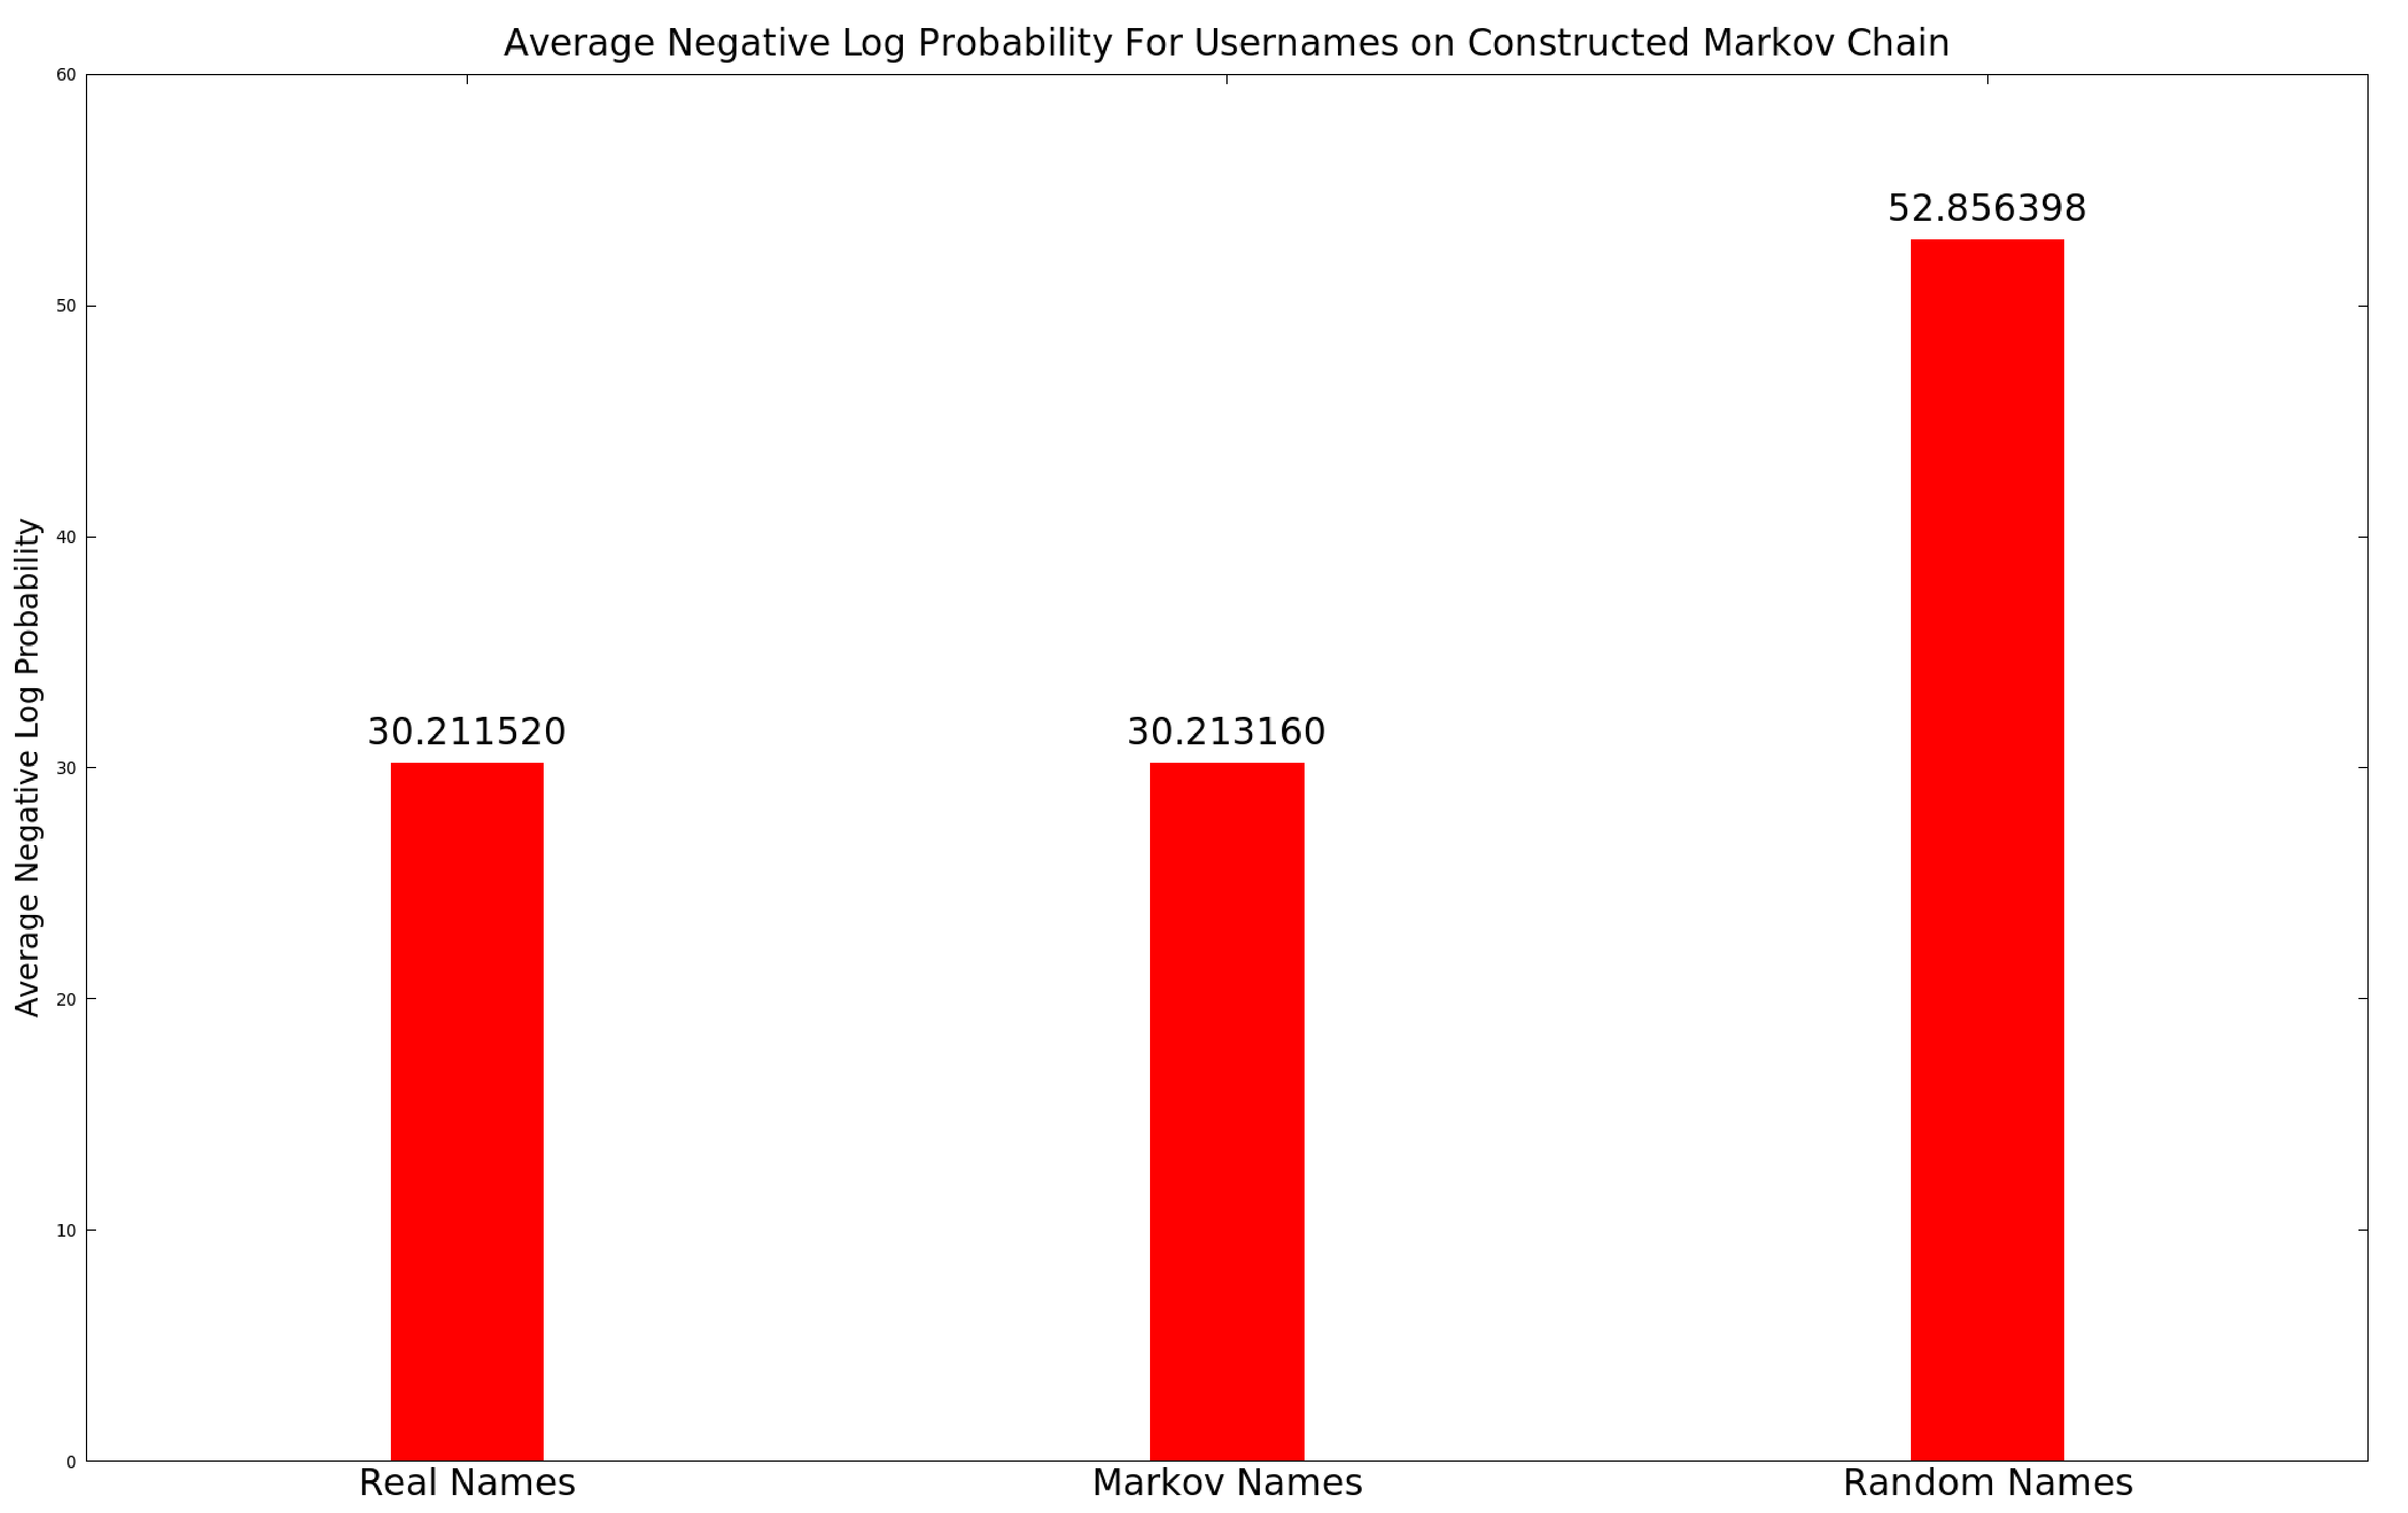
\includegraphics[width=\columnwidth]{usernames-average.eps}
\caption{Average negative log probability score for usernames based on constructed Markov chain.}
\label{fig:evaluation:usernames:average}
\end{figure}

\begin{table}
    \centering
		\resizebox {\columnwidth} {!} {
    \begin{tabular}{|lr|lr|lr|}
    \hline
    \multicolumn{2}{|l|}{Real Usernames} & \multicolumn{2}{l|}{Markov Chain Usernames}
    & \multicolumn{2}{l|}{Random Text Usernames} \\
    \hline
    Name & Score & Name & Score & Name & Score \\
    \hline
    davepeck & 20.189543 & Coccpthe & 24.123132 & wBc3HLqy & 44.472027 \\
    nytimes & 19.178421 & JorayLa & 17.191901 & gzQbhCT & 33.078578 \\
    focuspolitik & 31.618525 & beteckucovao & 30.477696 & KvJhlRwF4G45 & 67.152348 \\
    MarsHill & 20.768233 & Diajan\_m & 20.492829 & PthGonXE & 30.381789 \\
    Scobleizer & 26.922820 & Boumezzost & 25.873167 & vLdHuXVqDO & 56.543208 \\
    warrenellis & 24.335242 & shltirreaha & 30.877799 & 4ok1MwHzWD1 & 60.301202 \\
    redjumpsuit & 32.200608 & SEMarannesi & 25.831416 & QzFS7n4StQt & 58.562229 \\
    joshspear & 23.335631 & McolitePa & 23.613131 & ZhZ1B28vX & 46.774850 \\
    FUELTV & 21.209548 & tudwpi & 20.180779 & hFIn6O & 23.278177 \\
    fredwilson & 27.280397 & MarassttyM & 21.652989 & \_\_hKc4vhHi & 50.487769 \\
    \hline
    \end{tabular}
		}
    \caption{Sample names from each category and their scores.}
    \label{tab:evaluation:usernames:samples}
\end{table}

These results show that names generated by the Markov chain are statistically
identical (within 0.002) to the real usernames used to create the Markov chain.
It is unlikely that an automated system could distinguish between them.  Random
text, however, will not work in this case.  Randomly generated names appear
significantly different than real user names.

\subsubsection{Scoring Names using Human Analysis with Mechanical Turk}
\label{subsec:evaluation:usernames:mturk}

In addition to the statistical analysis, an experiment was performed using Amazon's
Mechanical Turk\footnote{\url{https://www.mturk.com}} system.  The Mechanical Turk
system is a way to connect experimenters that need a human to evaluate something
with willing participants that can perform the evaluation for a small fee per task.

For our experiment, we chose the sentiment analysis template.  This asks users
to choose from one of five choices and provides some more specific instructions
about each choice.  Each worker was shown one user name that is either a real user
name from Twitter, a name generated by our Markov chain, or a name that is just
random text.  The worker did not know from which group the name appeared.  

Essentially, we asked them to
score their confidence in recognizing whether or not the name was real.  If
they were confident that it was fake, they should have answered in the negative.
If they were confident that it was real, they should have answered in the positive.
If they were not sure, they should have answered neutral.  The negative responses
are scored with either -1 or -2 depending on their degree of confidence and the
positive responses are scored with either 1 or 2 depending on their confidence.
A neutral response scores 0.  Each worker was compensated \$0.10 for each name
they scored.  It should be noted that this experiment is exempt from IRB
approval because no identifying information about any participants is collected.
In fact, Mechanical Turk does not provide a way for requesters to identify workers.
Instead, each worker has a pseudonymous user ID number.  Participants were only
asked to respond to a survey of their opinions about the validity of the user names,
not even the user ID was collected after the experiment was performed.

In total, 50 names were chosen from each category and each name
was shown to five different workers.  The aggregated results are shown in figures
\ref{fig:evaluation:usernames:real-mturk-agg}, \ref{fig:evaluation:usernames:Markov-mturk-agg},
and \ref{fig:evaluation:usernames:random-mturk-agg}.  

\begin{figure*}
\begin{minipage}{0.3\textwidth}
        \centering
    \centering
    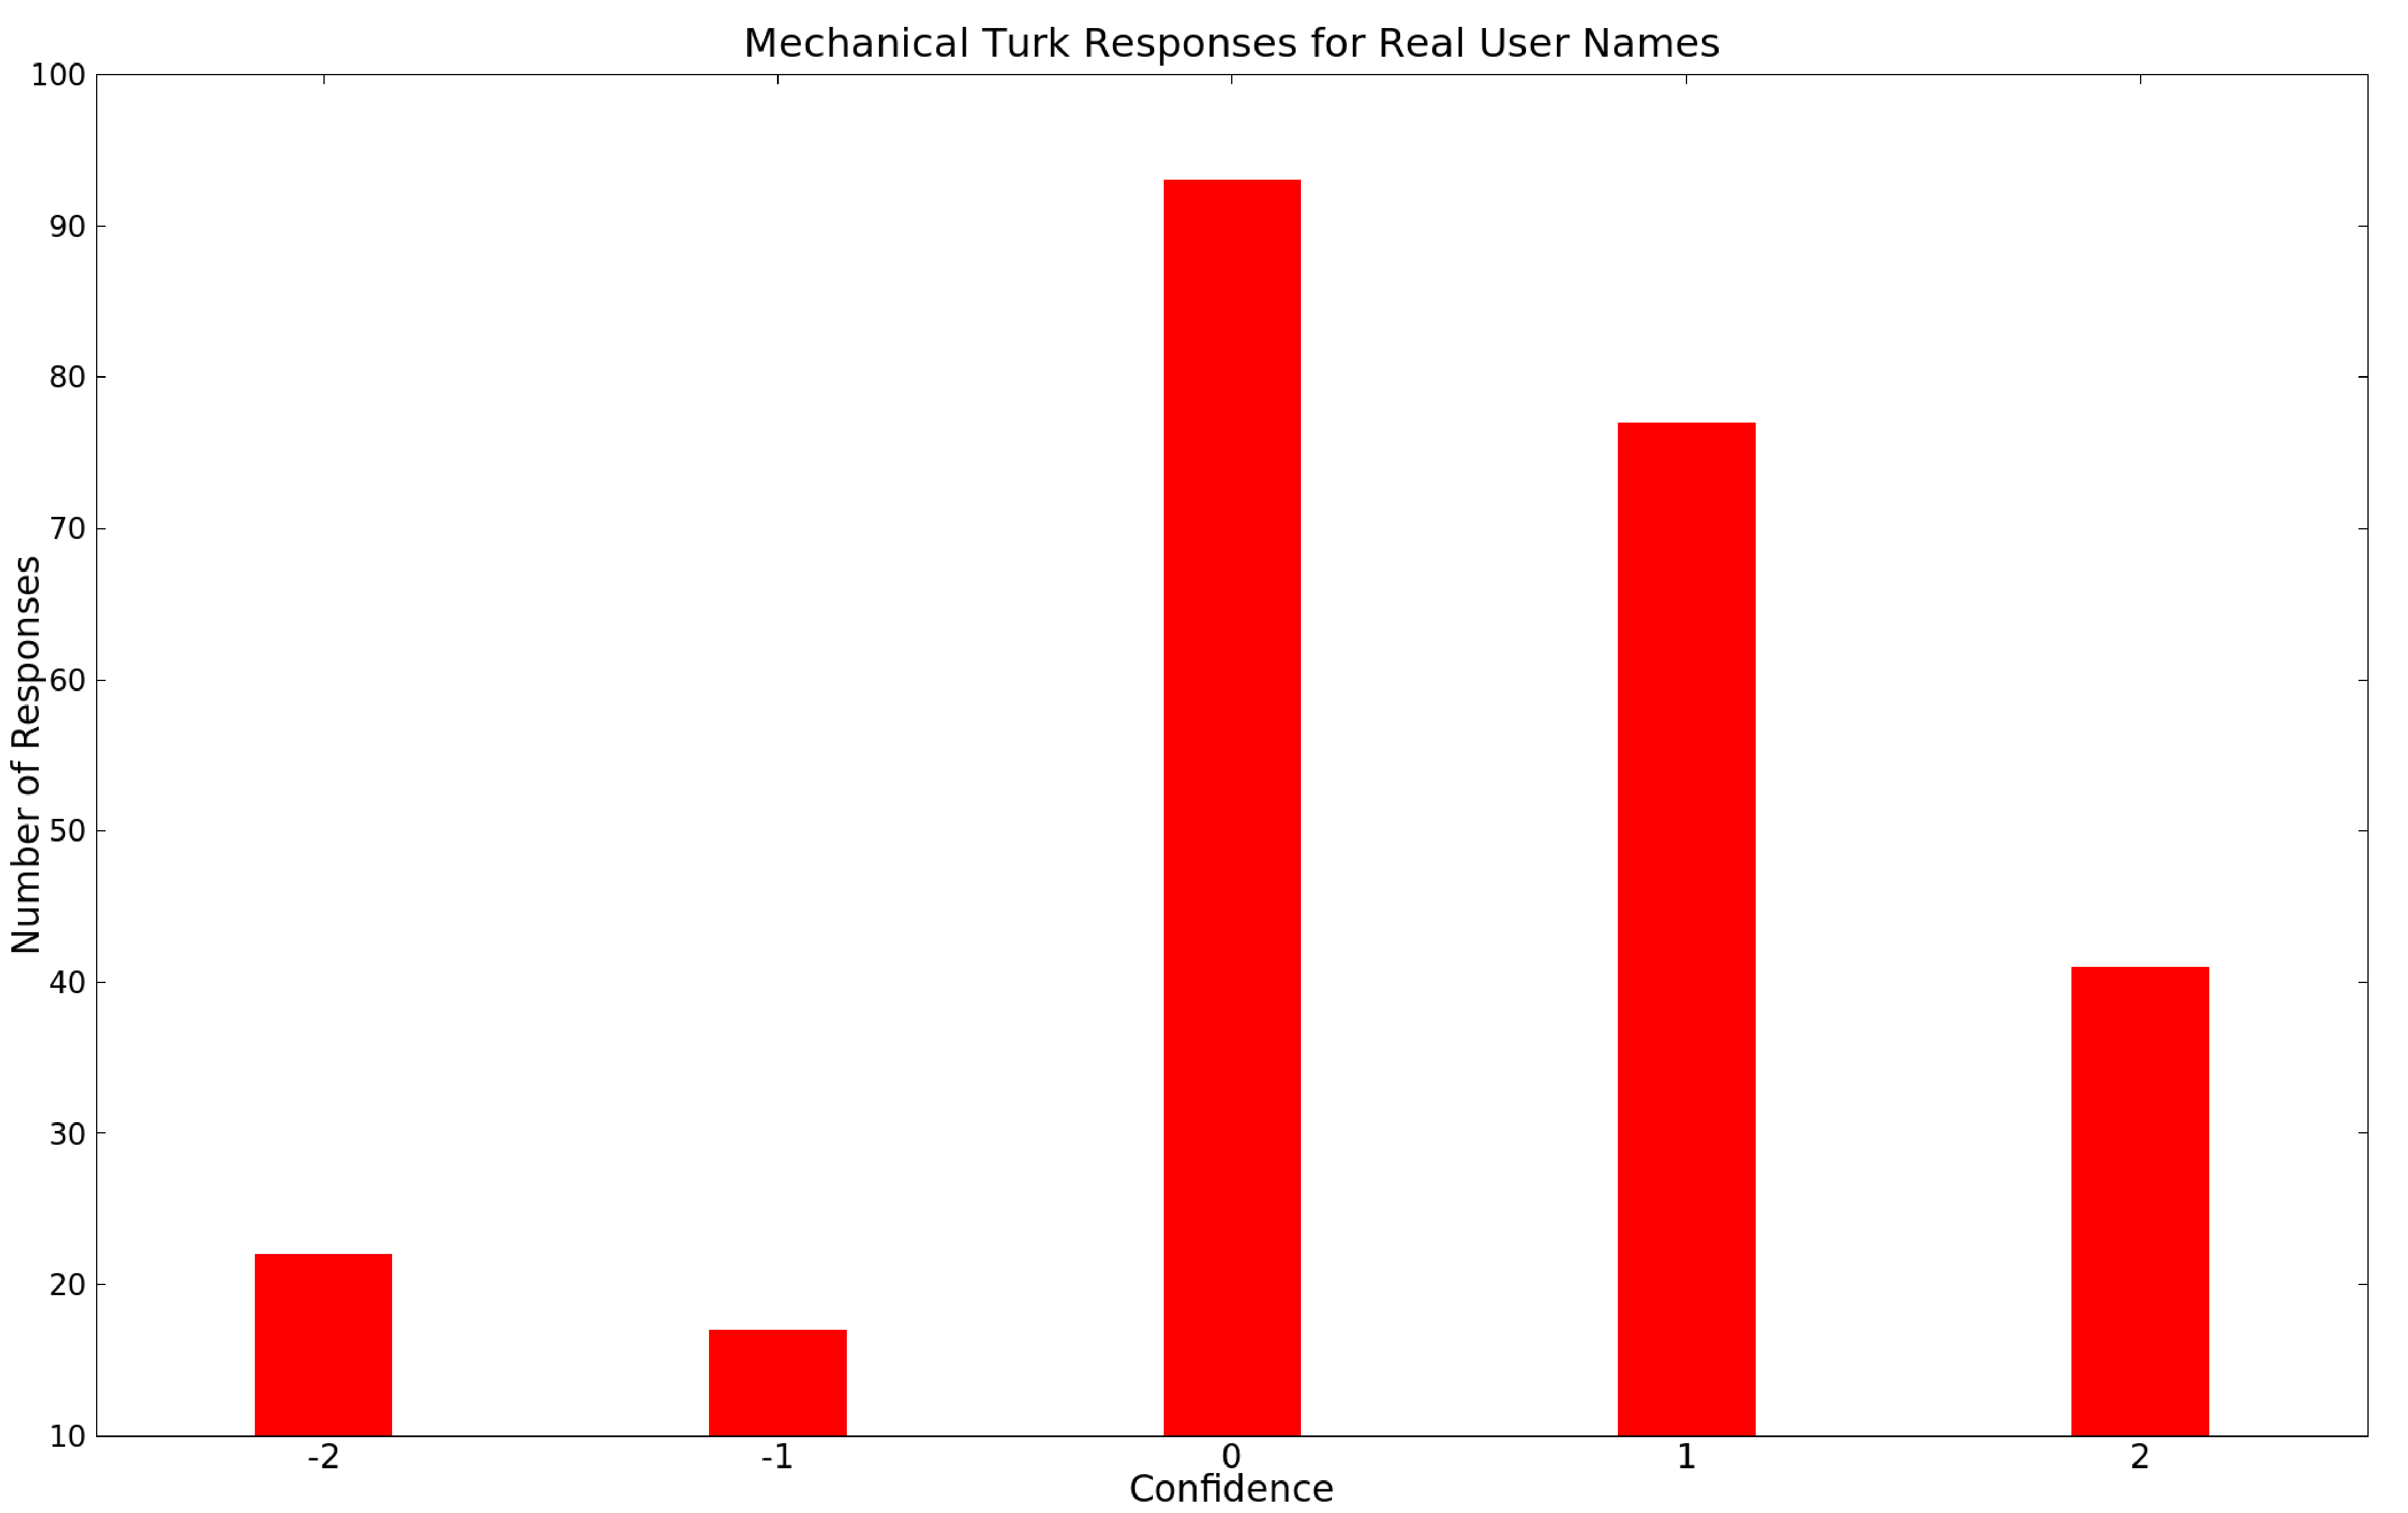
\includegraphics[width=\columnwidth]{real-mturk-agg.eps}
    \caption{Aggregate scores for real usernames from the Mechanical Turk experiment.}
    \label{fig:evaluation:usernames:real-mturk-agg}
\end{minipage}%
\hspace{5mm}
\begin{minipage}{0.3\textwidth}
        \centering
					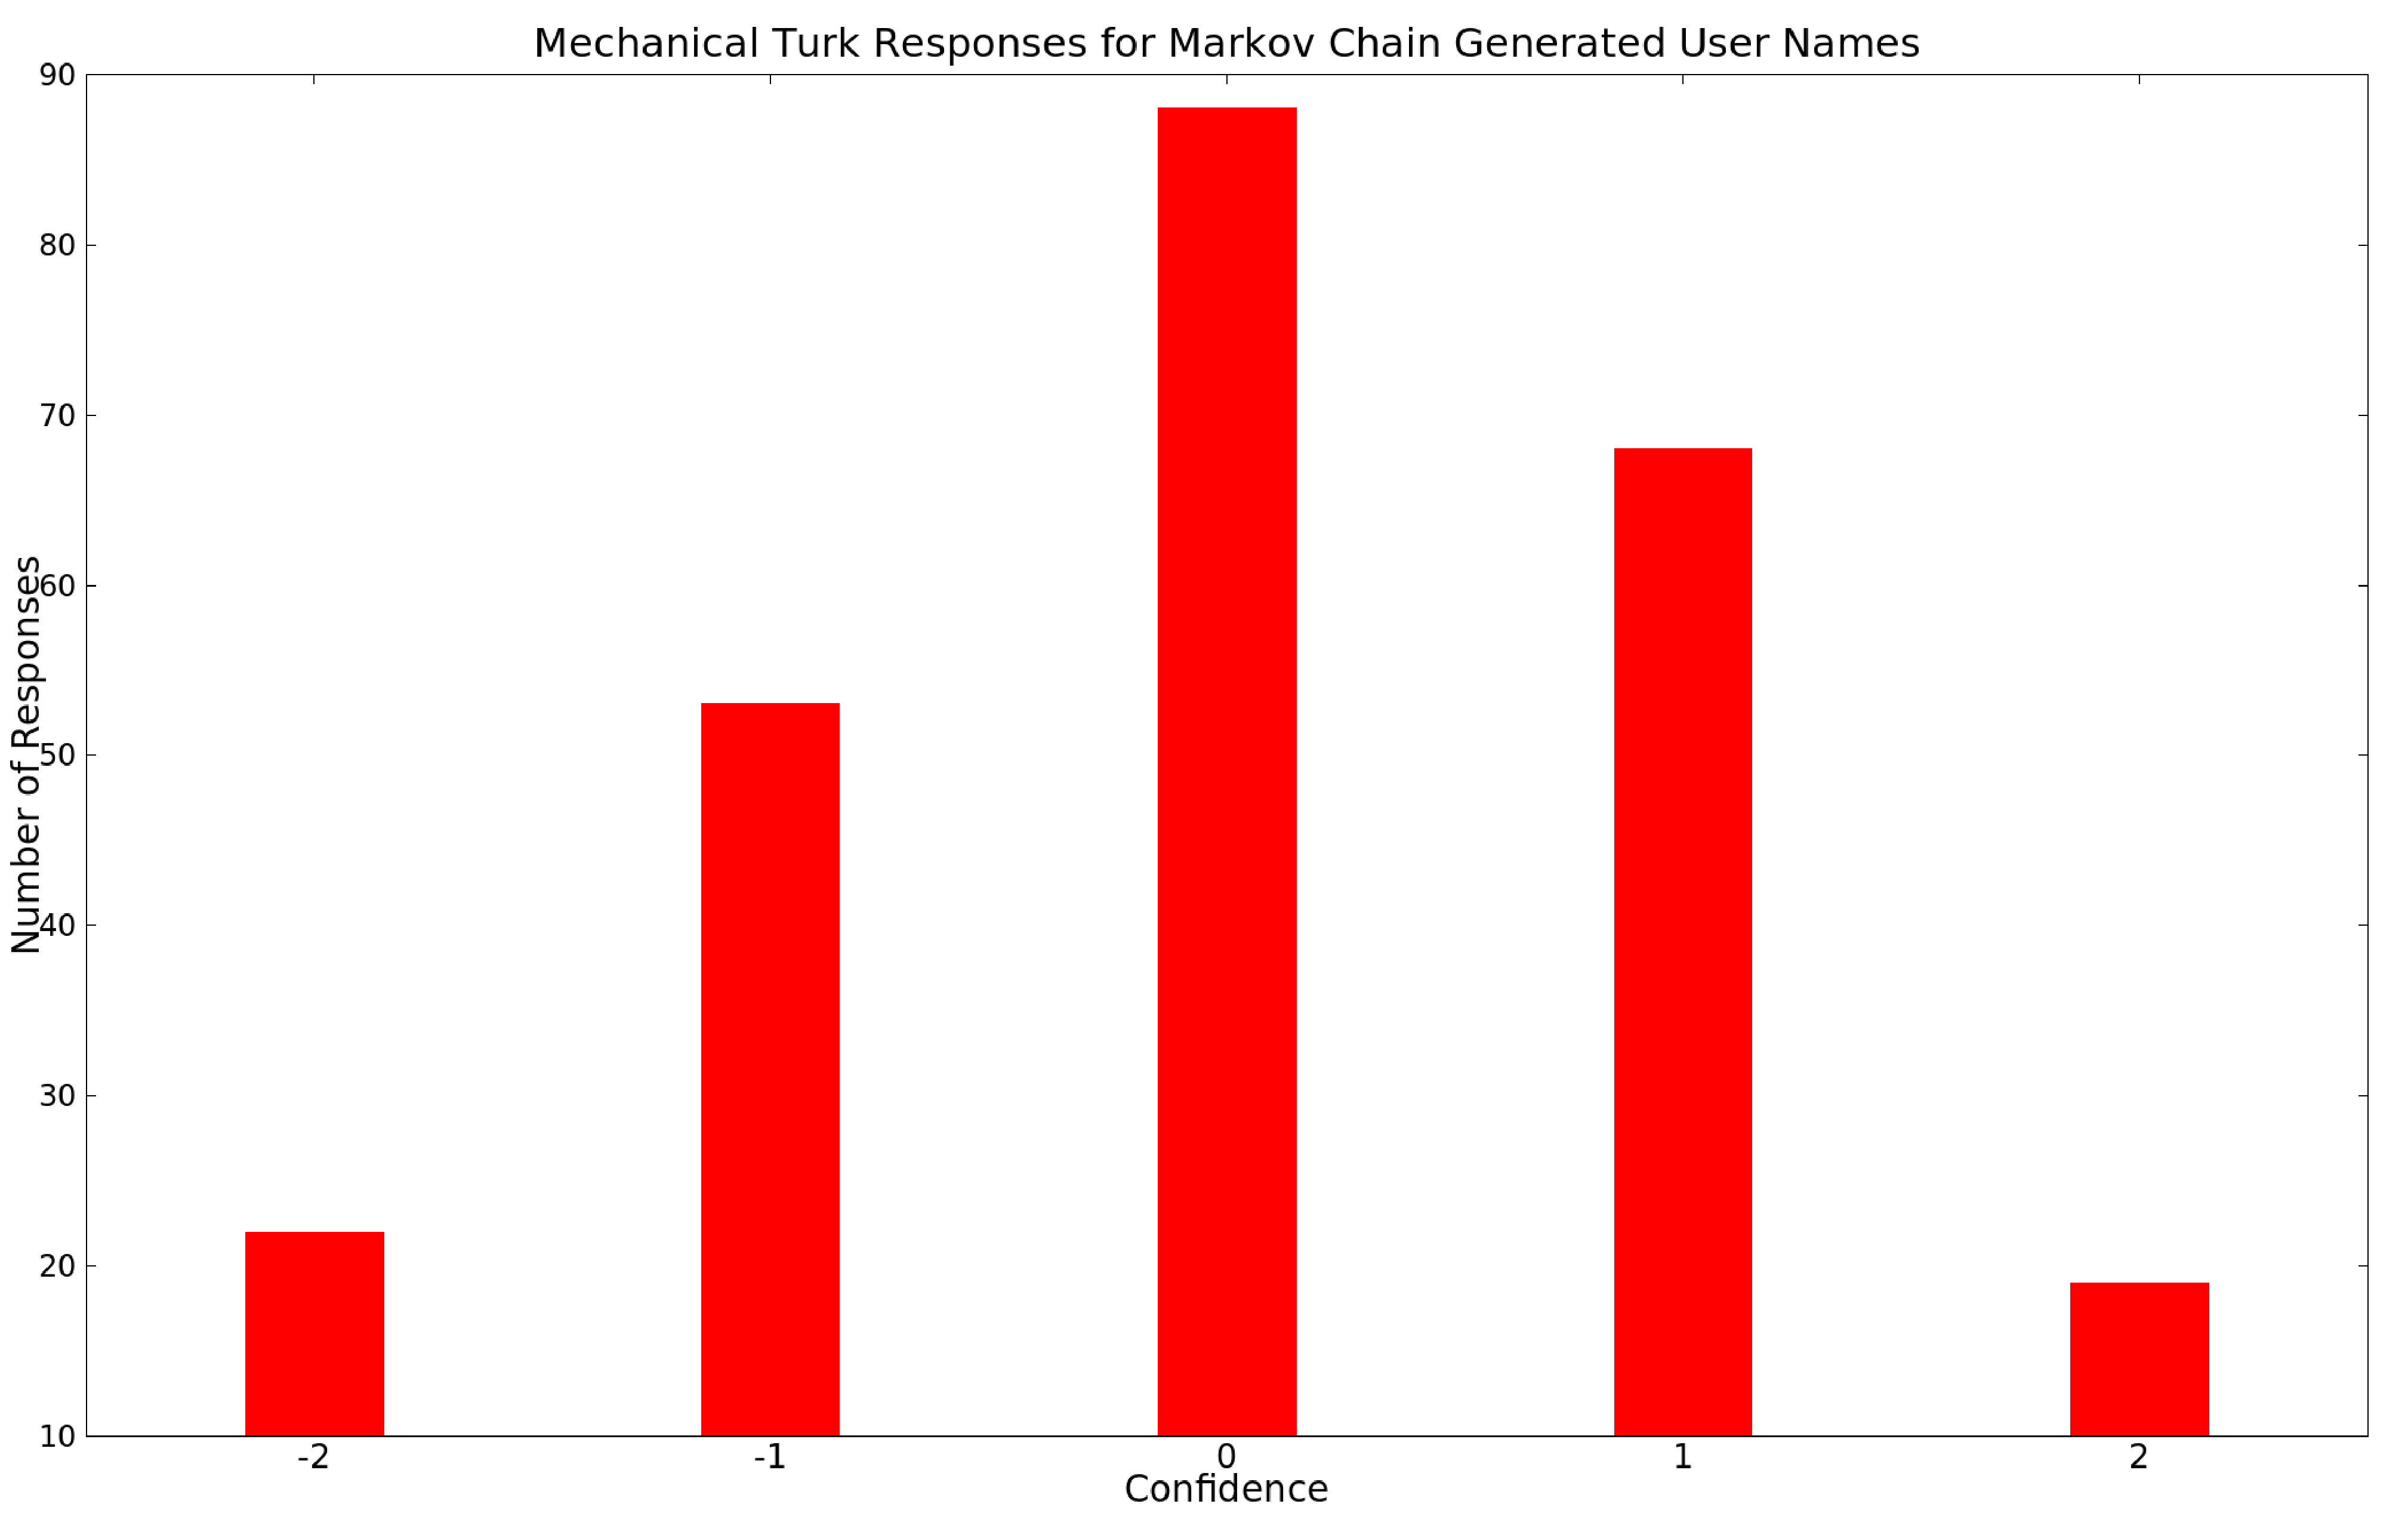
\includegraphics[width=\columnwidth]{Markov-mturk-agg.eps}
    \caption{Aggregate scores for Markov chain generated usernames from the Mechanical Turk experiment.}
    \label{fig:evaluation:usernames:Markov-mturk-agg}
\end{minipage}%
\hspace{5mm}
\begin{minipage}{0.3\textwidth}
        \centering
    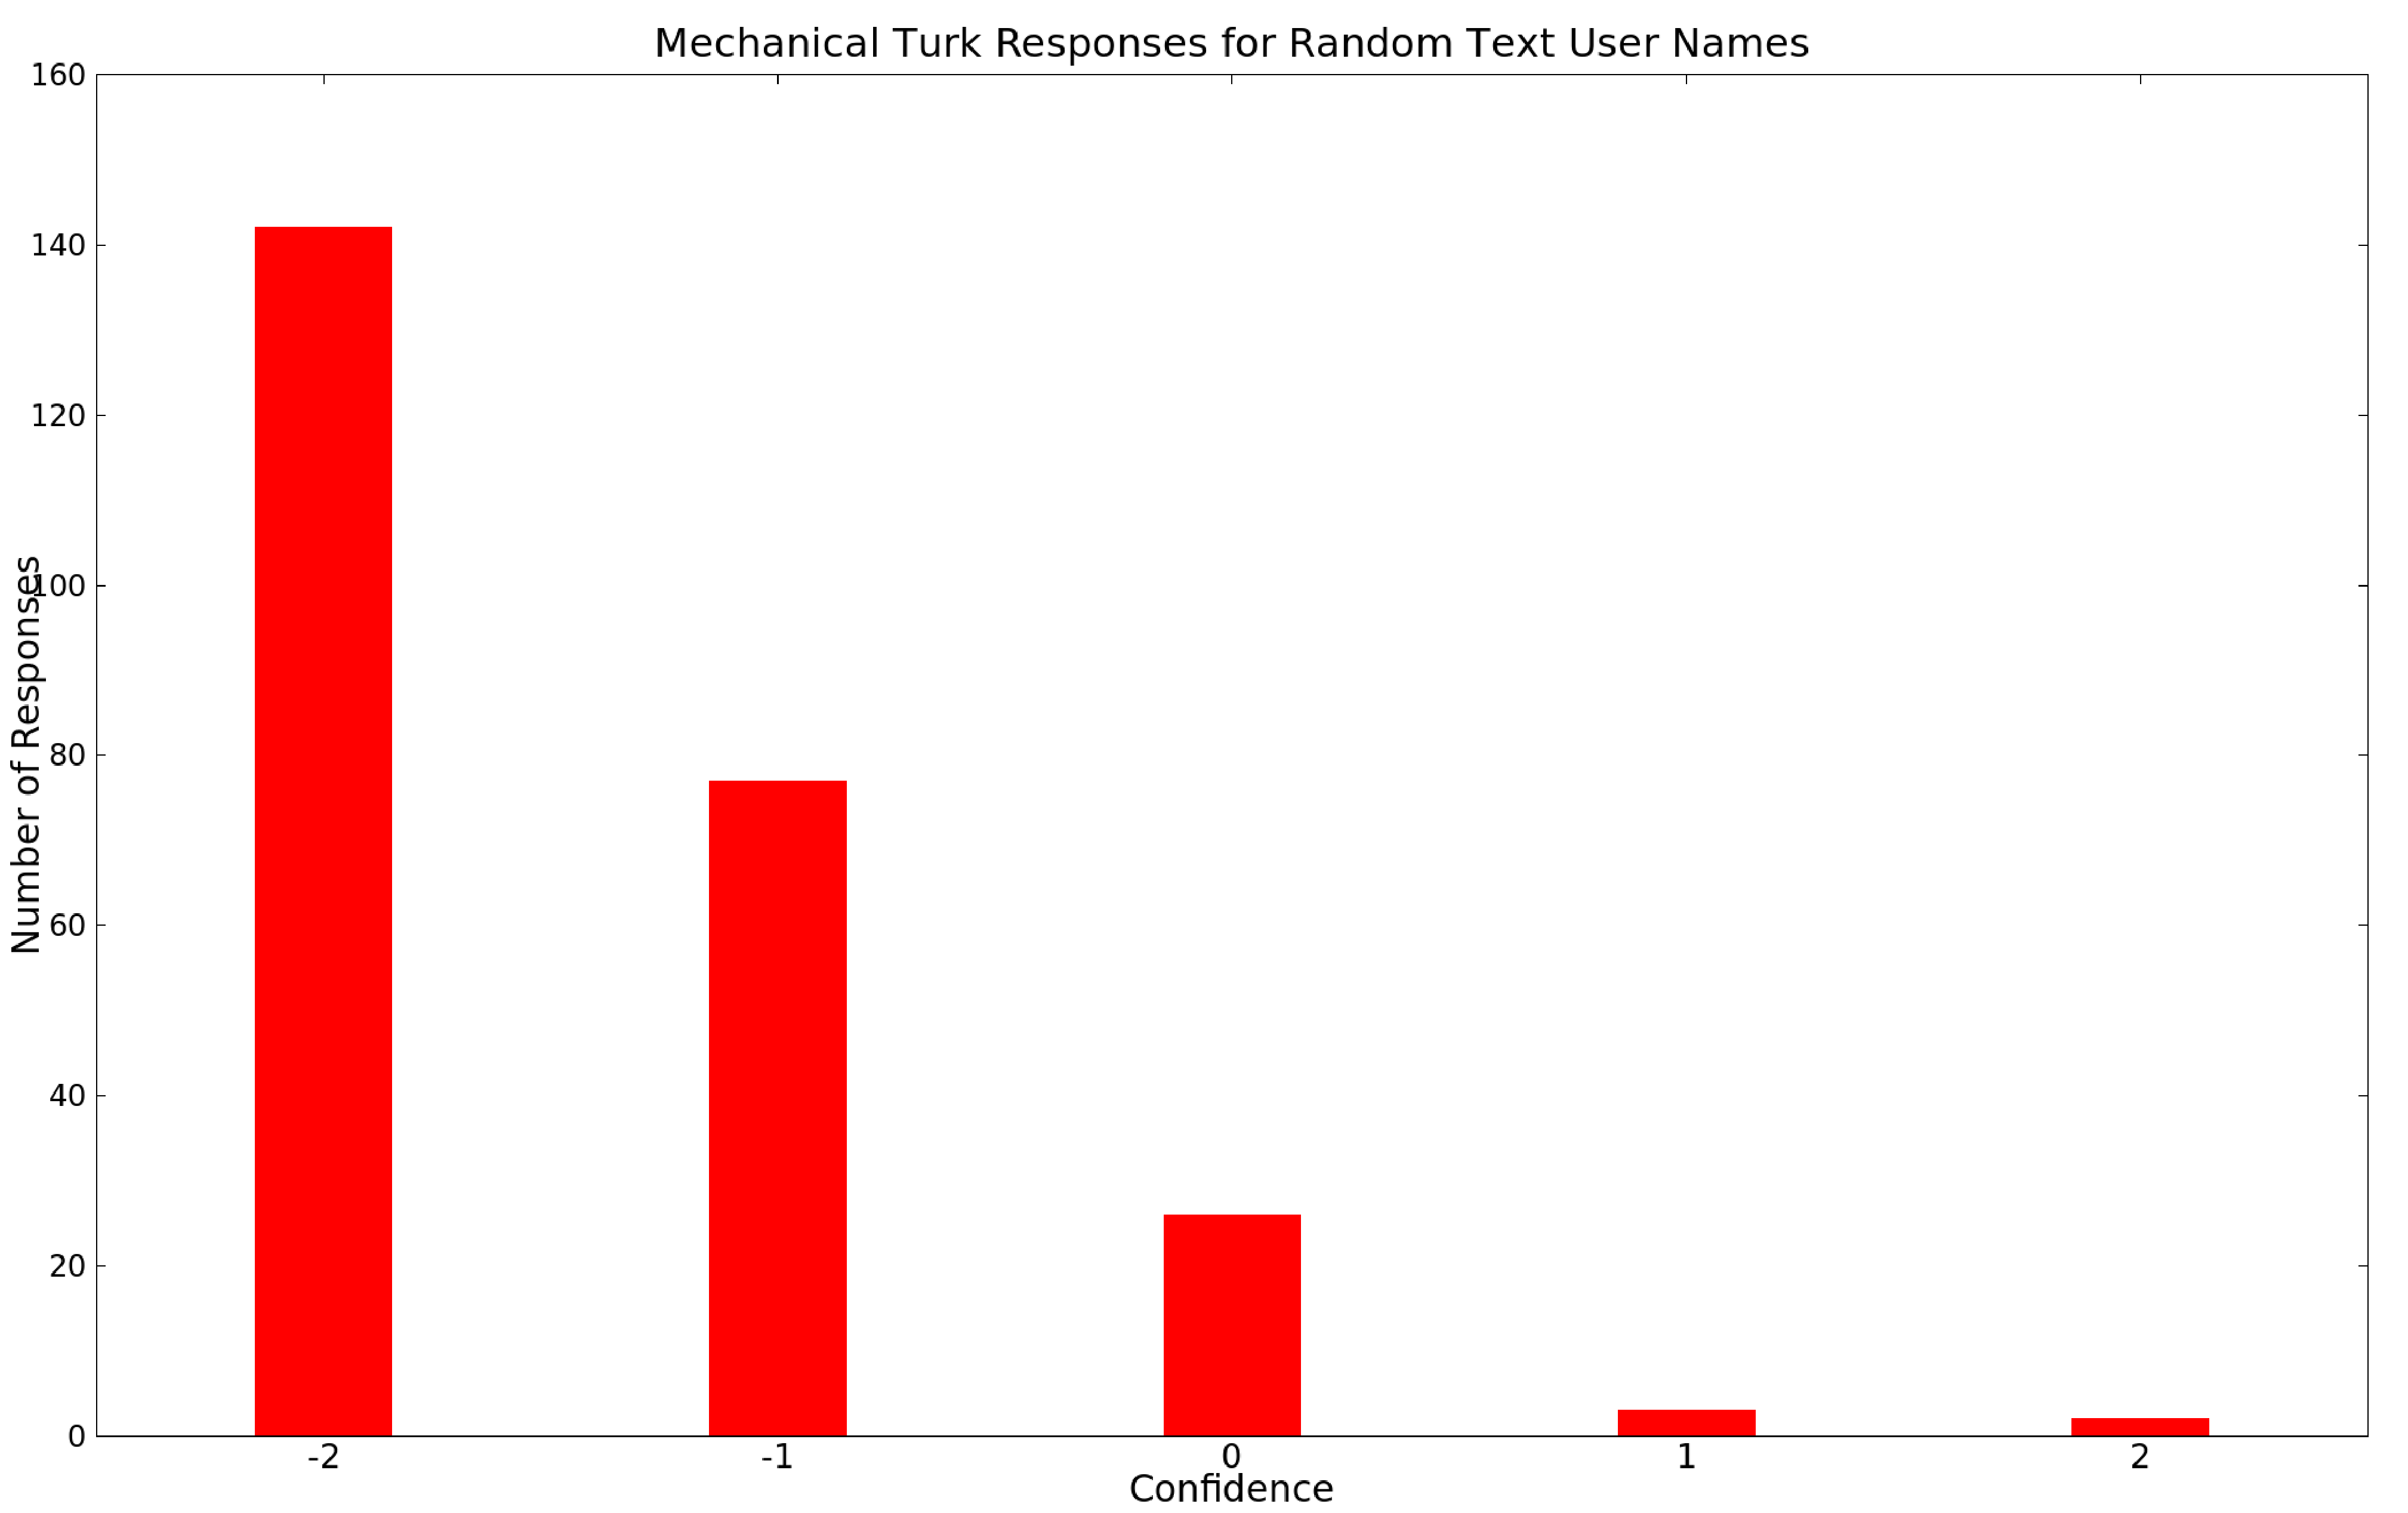
\includegraphics[width=\columnwidth]{random-mturk-agg.eps}
    \caption{Aggregate scores for random text usernames from the Mechanical Turk experiment.}
    \label{fig:evaluation:usernames:random-mturk-agg}
\end{minipage}
\end{figure*}

These results show some differences compared with the automated statistical
analysis above.  Random names, however, appear obviously fake to human examiners.
Almost all responses for the random names were negative.  It does appear, though,
that humans are not confident in recognizing real names either, with a plurality
of results being zero and some negative.  They seem to have some inclination toward
recognizing fake names generated by the Markov chain, with more negative answers
than the real user names, but very few considered themselves very confident (a score of -2).

The results from both the statistical analysis and the Mechanical Turk survey
indicate that the method being used for username generation is sufficient to
create usernames that would not appear abnormal to either an automated name
analysis tool or to human users viewing the page on Twitter.  Therefore, this
method can be used as the username generation method for a botnet that must
create a new account and switch communications to it for some reason, e.g.\ if
Twitter blocks the previous account.  By starting with a common seed, each bot
can generate the appropriate new name and connect to the new account.

\section{Related Work}
\label{subsec:lit-review:botnets:related-work}

Stegobot \cite{stegobot} is a botnet designed to communicate using
social networks (specifically Facebook) and image stegangraphy.  The authors
design two separated types of message: bot commands and bot cargo.  The bot
commands are messages from the botmaster to the bots instructing them.  The bot
cargo are messages from the bots back to the botmaster containing stolen
information.

Stegobot \cite{stegobot} uses a distributed, peer to peer communication channel
and does not generate its own cover messages.  Instead, it uses the image files that the
victims are already uploading to the social network as the cover messages,
embedding the secret messages within.  The botnet software intercepts the images
being posted to embed the message before it is sent to Facebook.  Stegobot uses
the existing network of relationships for each victim as the communication
channel.  In their experiments, the authors used a set of 116 images.  One of
the difficulties of this technique is the automatic image manipulation performed
by Facebook as the images are uploaded.  This can tamper with the content of the
embedded message, requiring a highly robust stego system.

Natarajan et al. \cite{stegobot-detect} designed a detection scheme for Stegobot
that uses the information entropy of the image files that are acting as the
cover objects.  Their detection technique achieved average detection rates
exceeding 70\% in their experiments for several different image steganography
methods.

A similar work by Singh et al. \cite{twitter-botnet} uses Twitter for
botnet C\&C, but does not apply steganography to hide the communications.
Instead, the commands are posted directly to the Twitter account.  This allows
the botmaster to leverage the benefits of social networks for botnet C\&C, but
they used communication methods that will likely appear highly suspicious to any
viewers.

SocialClymene \cite{socialclymene} is a detection scheme designed specifically
for detecting stego-based botnet command and control methods using social networks,
however it is designed for image steganography such as stegobot.  CatchSync
\cite{catchsync} is another detection technique that looks at connectivity of
nodes in a directed graph to find suspicious nodes.  In the case of Twitter,
connectivity is determined by which accounts follow other accounts.

Sebastian et al. \cite{graybot} have created a similar mechanism for botnet command and control
using encrypted tweets.  This method mixes irrelevant sentences among tweets
that contain botnet commands.  Their command tweets follow the formula of
\ttf{\#keyword command}, where the value of \ttf{command} would be encrypted.
While this method can hide the commands being issued, it does not conceal the
existence of the commands.  Each command follows the same formula and can be
differentiated from other tweets posted on the botmaster's account.  Additionally,
no mechanism is described for recovering if the botmaster's account has been
closed due to detection of malicious activity. 

\section{Conclusion}
\label{cha:conclusion}

In this paper, we have demonstrated a general-purpose stego system that allows secret communication through the
Twitter social network using only metadata for communication.  We have showed that this system can be used for
botnet command and control through the development of a Twitter stego system and a specialized botnet
C\&C language. 
We have discussed the performance evaluation of the proposed system using Emulab, 
and usability study using Amazon MTurk. We have also discussed how the vast 
userbase and large scale of Twitter facilitates ample steganograpic security.  
By demonstrating how a botmaster might perform
such communication using online social networks, our work provides the basis
to detect and prevent emerging botnet activities.

There are other possible steganographic techniques that can be applied using
Twitter.  For example, Twitter allows posting images along with
tweets\footnote{\url{https://support.twitter.com/articles/20156423-posting-photos-on-twitter}}
and there are many existing image steganography techniques \cite{watermarking}
that are often used for watermarking, but can also be used for communication.
The existing system can also be used on other social network websites such
as Facebook, but it may be necessary to collect data from these websites when
deciding on the message length distribution.  Unlike Twitter, these other
websites generally allow much longer posts, so the system could take advantage
of the increased variation.

It is possible to use this system for key exchange for other existing stego
systems.  It is necessary in steganographic key exchange to have a stego
system that can be used to transmit the key, otherwise an adversary can detect
the communication of the keys.  Because this system has a relatively low
information bandwidth, it may be well suited for key exchange that does not
require a significant amount of information.  This concept is applied in
cryptography where a public key algorithm such as RSA is used to send a
key for a symmetric algorithm such as AES because AES can achieve better
encryption and decryption performance than RSA, although it is technically
possible to send all of the communications using RSA.


\bibliographystyle{plain}
\bibliography{biblio}{}

\end{document}
